%%%%%%%%%%%%%%%%%%%%%%%%%%%%%%%%%%%%%%%%%%%%%%%%%%%%%%%%%%%%%%%%%%%%%%
%%                                                                 %%
%% Please do not use \input{...} to include other tex files.       %%
%% Submit your LaTeX manuscript as one .tex document.              %%
%%                                                                 %%
%% All additional figures and files should be attached             %%
%% separately and not embedded in the \TeX\ document itself.       %%
%%                                                                 %%
%%%%%%%%%%%%%%%%%%%%%%%%%%%%%%%%%%%%%%%%%%%%%%%%%%%%%%%%%%%%%%%%%%%%%

\documentclass[sn-mathphys,Numbered]{sn-jnl}  % If you add `lineo` to have linenumbers here, you cannot skip linenumbering in tables

%%%% Standard Packages
%%<additional latex packages if required can be included here>
\usepackage{graphicx}%
\usepackage{multirow}%
\usepackage{amsmath,amssymb,amsfonts}%
\usepackage{amsthm}%
\usepackage{mathrsfs}%
\usepackage[title]{appendix}%
\usepackage{xcolor}%
\usepackage{textcomp}%
\usepackage{manyfoot}%
\usepackage{booktabs}%
\usepackage{algorithm}%
\usepackage{algorithmicx}%
\usepackage{algpseudocode}%
\usepackage{listings}%

%%%%
% REMOVE THOSE IN THE END
\usepackage{todonotes}
\usepackage{caption}
\usepackage{tabularx}
\usepackage{adjustbox}  % for the adjustwidth
\usepackage{threeparttable}  % to support notes within a table
\usepackage{makecell}  % For \makecell command

\usepackage{capt-of}
\usepackage{subcaption} % for subtables


\renewcommand\theadfont{\bfseries}



%\jyear{2021}%

\theoremstyle{thmstyleone}%
\newtheorem{theorem}{Theorem}%  meant for continuous numbers
\newtheorem{proposition}[theorem]{Proposition}% 
\theoremstyle{thmstyletwo}%
\newtheorem{example}{Example}%
\newtheorem{remark}{Remark}%
\theoremstyle{thmstylethree}%
\newtheorem{definition}{Definition}%
\raggedbottom


\newcommand{\microbetag}{\texttt{microbetag}}

\usepackage{lineno}
\newenvironment{mytable}
{
    \nolinenumbers
    \begin{table}[ht]
    \centering
}
{
    \end{table}
    \linenumbers
}



\begin{document}

% \linenumbers

\title[Article Title]{
    % Genomic, metabolic and literature oriented annotation of microbial co-occurrence networks enhances associations confidence level and hypothesis generation
    microbetag: simplifying microbial network interpretation through annotation, enrichment and metabolic complementarity analysis
}


%%==================================%%
%% Authors - affiliations           %%
%%==================================%%


\author[1]{\fnm{Haris} \sur{Zafeiropoulos}}\email{haris.zafeiropoulos@kuleuven.be}
\author[1]{\fnm{Ermis Ioannis} \sur{Michail Delopoulos}}\email{ermisioannis.michaildelopoulos@student.kuleuven.be}
\author[2]{\fnm{Andi} \sur{Erega}}\email{andi.erega@hest.ethz.ch}
\author[2]{\fnm{Annelies} \sur{Geirnaert}}\email{annelies.geirnaert@hest.ethz.ch}
\author[3]{\fnm{John} \sur{Morris}}\email{scooter@cgl.ucsf.edu}
\author*[1]{\fnm{Karoline} \sur{Faust}}\email{karoline.faust@kuleuven.be}


\affil*[1]{
    \orgdiv{
        Department of Microbiology, Immunology and Transplantation, Rega Institute for Medical Research
    }, 
    \orgname{KU Leuven}, 
    \orgaddress{
        \street{Herestraat}, \city{Leuven}, \postcode{3000}, \state{}, \country{Belgium}
    }
}

\affil[2]{
    \orgdiv{Institute of Food, Nutrition and Health}, 
    \orgname{ETH Zurich}, 
    \orgaddress{
        \street{Street}, \city{Zurich}, \postcode{8092}, \state{}, \country{Switzerland}
    }
}

\affil[3]{
    \orgdiv{Department of Pharmaceutical Chemistry}, 
    \orgname{University of California San Francisco}, 
    \orgaddress{
        \street{Street}, \city{San Francisco}, \postcode{94143}, \state{California}, \country{USA}
    }
}

%%==================================%%
%% unstructured abstract %%
%%==================================%%
\abstract{

    % Up to 350 words.
    
    \textbf{Background:} 
    % the context and purpose of the study
    The inference of microbial association networks from metagenomic data is a popular hypothesis-generating method, yet its use is hampered by low accuracy and tool dependency “Reverse ecology” uses genomic and metabolic modeling to predict ecological traits for less well-known microorganisms and their interactions within microbial communities.  
    microbetag combines reverse ecology approaches with phenotypic trait mapping to ease the interpretation of microbial association networks.

    \textbf{Results:} 
    % the main findings

    microbetagDB consists of $34,608$ high-quality Genome Taxonomy DataBase genomes, along with their corresponding KEGG annotations and genome-scale metabolic reconstructions. Seed sets (externally acquired compounds) were retrieved from the latter, supporting the prediction of over 1 billion potential pairwise metabolic interactions. 
    Relying on KEGG MODULE definitions, $342,000$ unique pathway complements were identified based on pairwise overlaps between the annotated genomes. 
    In addition, 33 phenotypic traits (e.g., pH optima, oxygen tolerance etc.) were predicted for the annotated genomes and incorporated in microbetagDB. 
    microbetag maps node taxonomies to their closest genome in microbetagDB and annotates them with phenotypic traits and functional potential previously derived from the literature. 
    Edges are then annotated with pathway complements and seed complementarities that may represent cross-feeding relationships. 

    In a validation case, microbetag successfully identified potential metabolic interactions between  \textit{Variovorax} and neighboring species, enabling the latter to produce thiamine in a network derived from a mining waste microbial consortium. .... 

    Accessible as a CytoscapeApp, microbetag offers a user-friendly interface called microbetag GUI (MGG) that simplifies the construction of a fully annotated co-occurrence network from an abundance table, providing a quick and intuitive way to explore hypotheses about microbial interactions. 


    \textbf{Conclusions:} 
    % a brief summary and potential implications
    microbetag, together with its database and GUI, simplify the interpretation of microbial association networks by systematically integrating prior knowledge about the taxa involved. 

%  =============================================================

    \begin{figure}[H]
        \label{fig:abstract}
        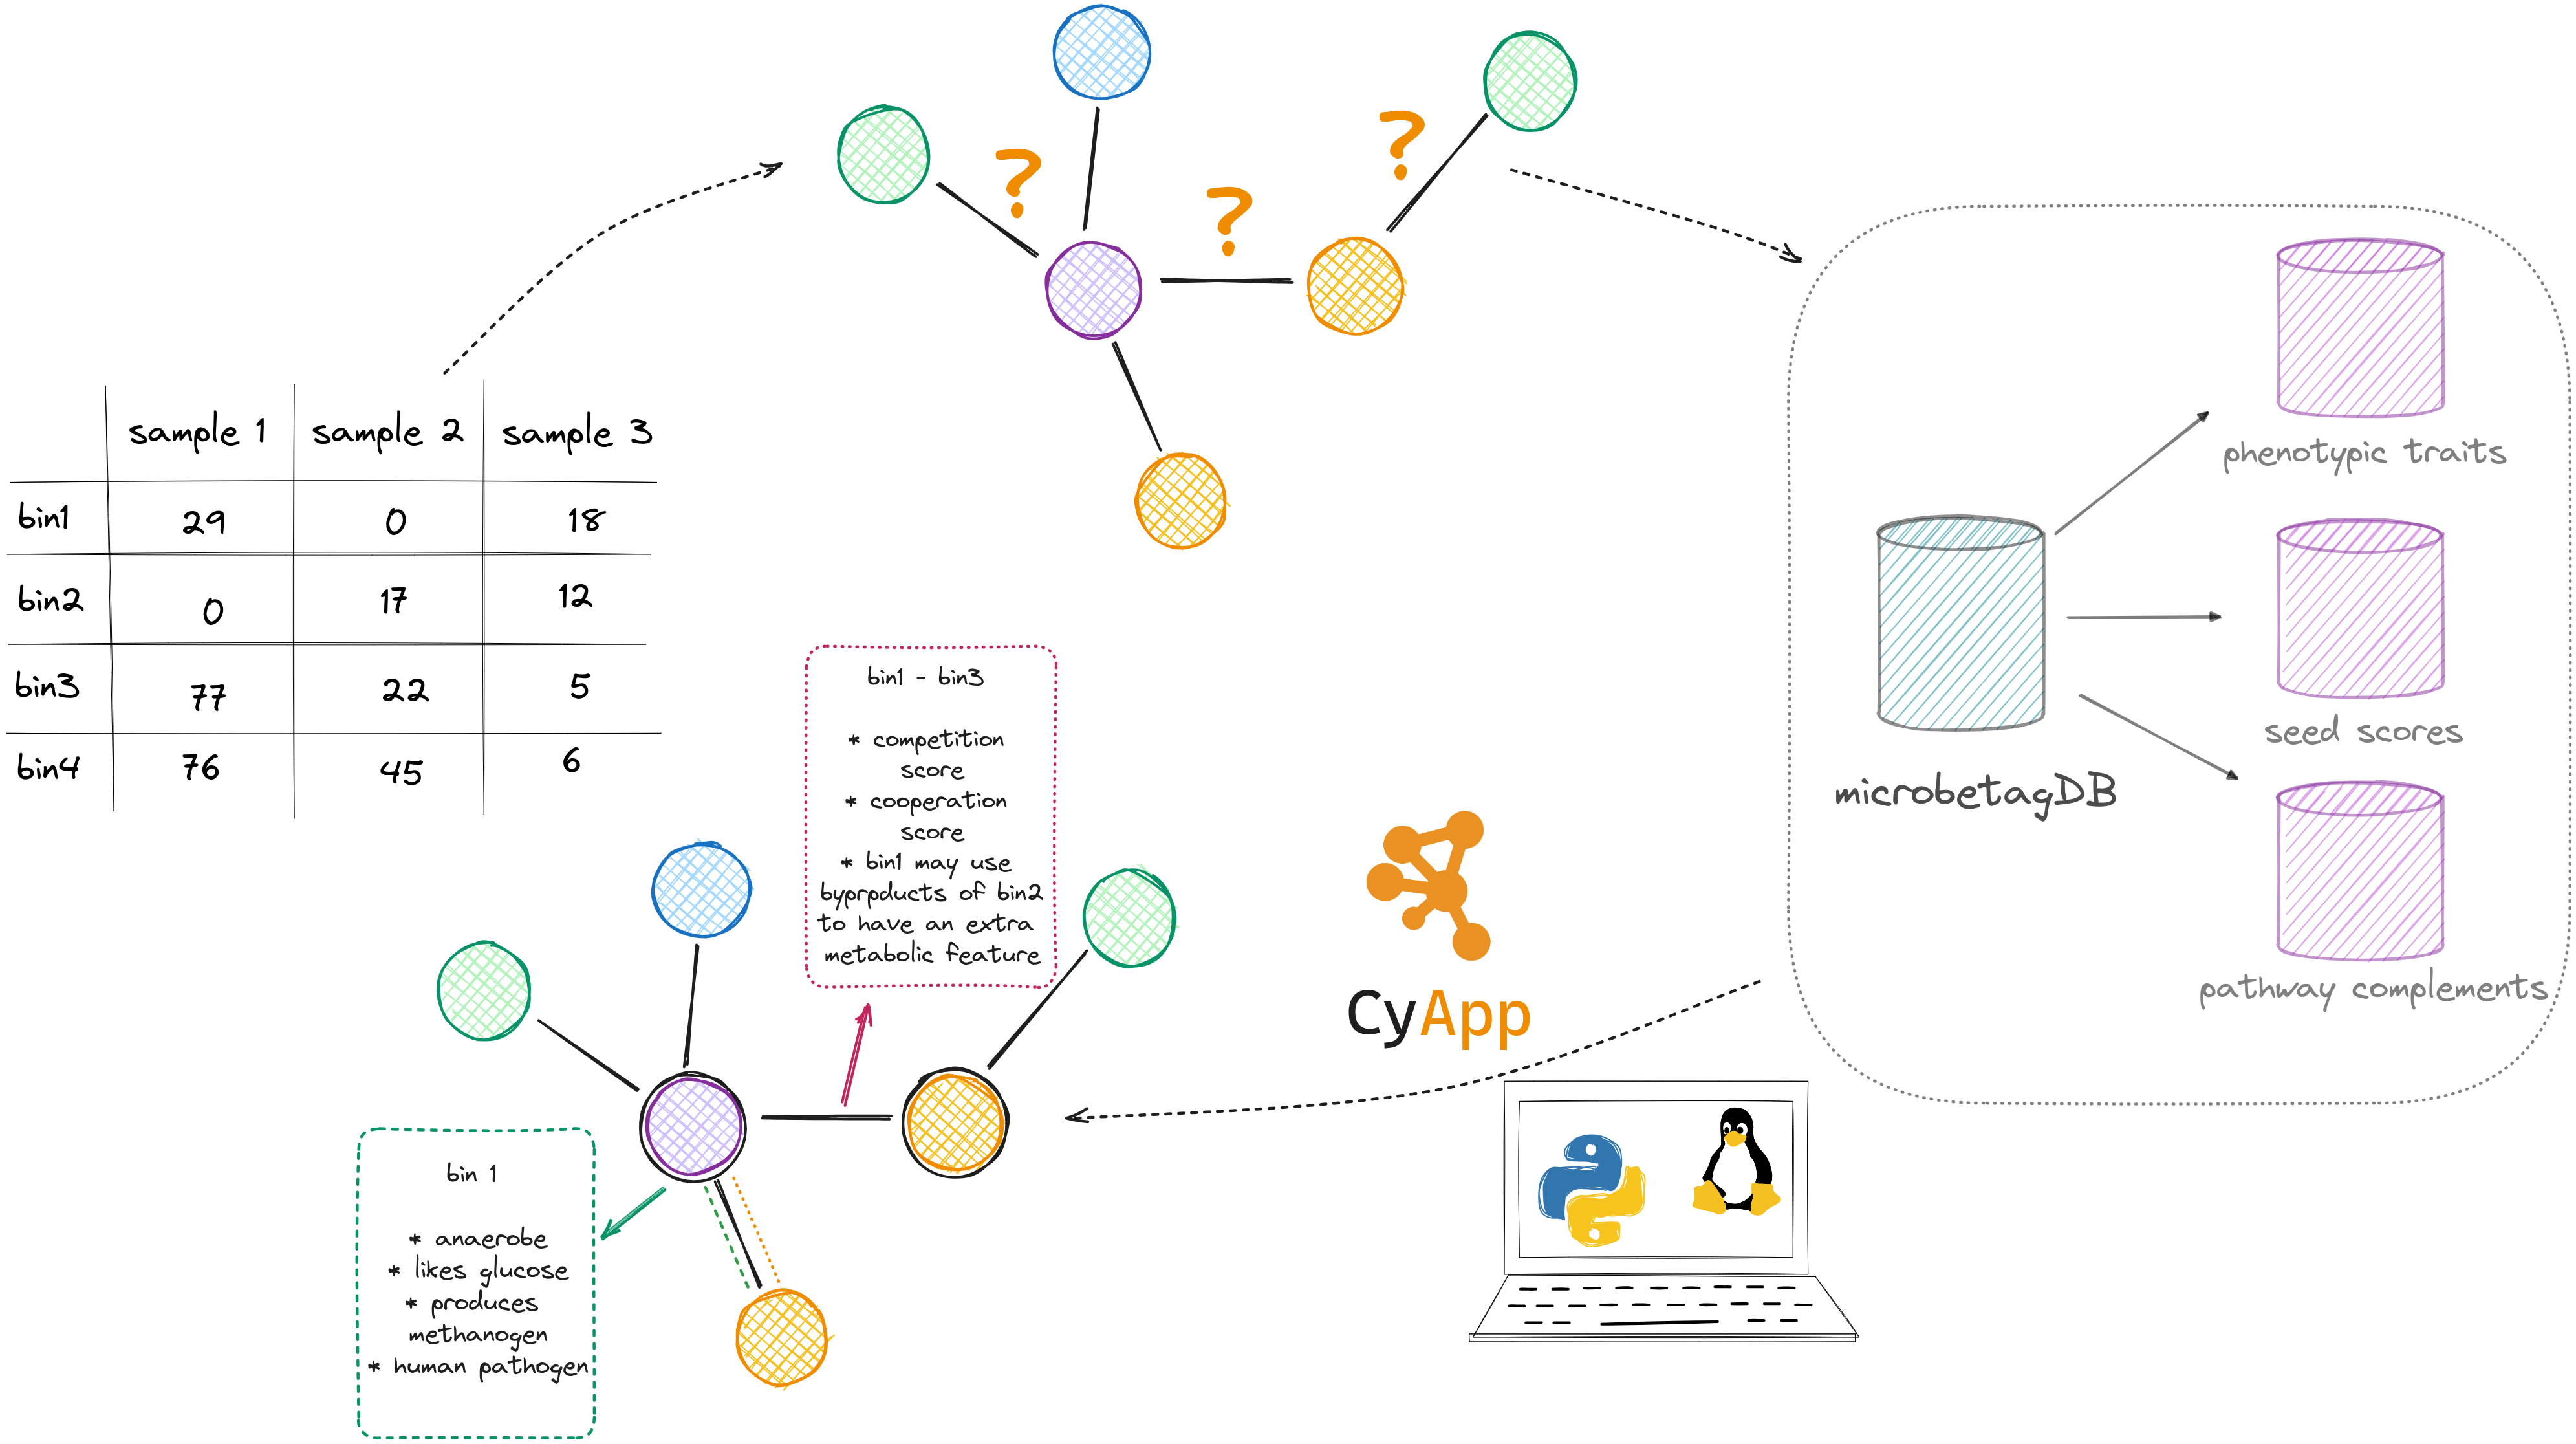
\includegraphics[width=\columnwidth]{figs/figure_abstract.png}
        \caption*{
            Figure abstract. 
            
            % From a count table (bins or OTUs/ASVs) one can come up with a co-occurrence network. 
            % To better understand and assess the confidence level of these associations, microbetag annotates both taxa (nodes) 
            % and 
            % integrating 
            % genomic data 
            
        }
    \end{figure}

}
%%==================================%%
%% keywords                         %%
%%==================================%%
\keywords{
    microbial associations,
    enrichment analysis,
    data integration,
    pathway complementarity,
    seed set
}

\maketitle


%%==================================%%
%% MAIN BODY                        %%
%%==================================%%


% ====================================================
% Background
% ====================================================
% REMEMBER: To have a footnote in the \section{}, you need to have NO empty lines; otherwise latex will not compile
\section*{Background}
\label{sec:background}

    % \footnote{
    % We are to submit in the Microbiome journal as a "Software" manuscript, thus we follow~\href{https://microbiomejournal.biomedcentral.com/submission-guidelines/preparing-your-manuscript/software-article}{these rules}.
    % }
    % \footnote{
    % The Background section should explain the relevant context and the specific issue that the software described is intended to address.
    % No subheadings.
    % }

    Microbial interactions play a fundamental role in the stability and resilience of ecosystems and their processes; from soils, aquatic environments and biogeochemical cycles~\cite{yuan2021climate} to host-associated environments and the human health~\cite{raes2008molecular, faust2012microbialReviewInteractions}.
    Most microbial species live only in communities~\cite{rottjers2018hairballs} and most natural microbial communities consist of hundreds or even thousands of species~\cite{balint2016millions}.
    Each species exhibits a unique repertoire of reactions and adapts to various niches, each with specific nutrient and environmental requirements.
    % Understanding the dynamics governing interactions among microbial species and their relationships with the surrounding environment would shed light on several aspects microbial ecology~\cite{robinson2010structure}.
 
    % references if we'd like to talk about microb com as ~\textit{complex systems}: ~\cite{godfray1990complex, amor2017spatial},

    % KF: what is the link of all this to microbetag? I suggest to strongly reduce this part
    % HZ: I remove the paragraph regarding the taxonomic vs functional variability; I had an idea on that but it would get too long to get there.. 
    %       For the paper we were discussing reg. an analysis on microbetagDB data this might be a nice question to ask! :)    
    % KF: and write instead more about:
    %        interaction mechanisms and 
    %        why it is so difficult to infer interactions from abundance data
    Depending on the net fitness effects that result for the taxa involved, interactions range from cooperation, competition, parasitism, commensalism and amensalism~\cite{faust2012microbialReviewInteractions}.
    Metabolic interactions can be established through a range of contact-independent and contact-dependent mechanisms leading to both positive and negative interactions. 
    These interactions can involve either one-way (unidirectional) or two-way (bidirectional) exchanges of metabolites.
    Depending on the biosynthetic cost borne by the interacting partners, two types of metabolite exchanges occur: by-product cross-feeding, where metabolites result from a selfish act of the producer, and cooperative cross-feeding, where one partner actively invests resources to produce metabolites benefiting the interaction partner~\cite{d2018ecology}.


    High-throughput sequencing (HTS) has provided insight into the diversity and composition of microbial communities~\cite{elixir_microbiome}. % get more refs
    Uncultivated species can now be detected, and their features can be inferred through their genomic information~\cite{hug2016new}.
    Moreover, the composition of thousands of microbiome samples is now accessible allowing for the inference of patterns among sets of samples.
    A widely used approach to extract such patterns is the creation of co-occurrence networks based on metagenomic read data (amplicon and/or shotgun)~\cite{matchado2021network}. 
    Several approaches are available for co-occurrence network inference based on a range of statistical concepts such as: correlation (e.g., CoNet~\cite{faust2012microbial}, SparCC~\cite{friedman2012inferring}), linear regression (e.g., SpiecEasi~\cite{kurtz2015sparse}) and indirect causal inference (FlashWeave~\cite{flashweave_cite}).
    % instead of indirect causal inference, one could say "conditional dependency identification"
    Nevertheless, microbial co-occurrence networks continue to encounter various challenges~\cite{faust2021open, cao2017inferring}.
    % Their inference inherits the challenges of metagenomic data analysis (e.g., compositionality, parameters inference)~\cite{cao2017inferring}.
    Each inference approach comes with its own assumptions and parameterization, leading to variations in network structure. 
    The choice of correlation metrics, the data preprocessing techniques applied and the handling of sparsity and zero inflation, and considerations for indirect causal relationships all influence the resulting network~\cite{cao2017inferring}. 
    As a consequence, the result of network construction is tool-dependent~\cite{kishore2023inferring, weiss2016correlation}.
    Moreover, their inference inherits the challenges of metagenomic data and analysis (e.g., sampling scale, compositionality, parameters tuning) and the returned network is a "hairball" of densely interconnected taxa.
    Thus, additional analysis is necessary to generate testable hypotheses~\cite{faust2021open}.
    Addressing the question of~\textit{What can we learn from the hairballs} posed by R{\"o}ttjers et \textit{al.}~\cite{rottjers2018hairballs} could provide insight into the mechanisms of the interactions.

    % KF: why has the use of network inference for interaction prediction underscored its limited accuracy? Imprecise expression: the use itself did not underscore the low accuracy - evaluations did. This needs to be rephrased.
    % HZ: How about now ?
    The assessment of interaction predictions derived from microbial co-occurrence networks has underscored their low accuracy for this task~\cite{berry2014deciphering, guo2022microbial, ma2020earth}.
    % Theoretical principles derived from network studies might provide indications of emergent biological characteristics~\cite{rottjers2018hairballs, guo2022microbial}. 
    % For example, modules (highly interconnected nodes) within microbial co-occurrence networks could serve as indicators of ecological processes that govern community structure, including niche filtering and habitat preference~\cite{ma2020earth}.
    Data integration and clustering have been suggested to address this challenge~\cite{faust2021open}.
    Clusters identified in microbial association networks have demonstrated their ability to mirror key drivers of community composition~\cite{guidi2016plankton} and several algorithms and implementations are available~\cite{rottjers2020manta}.
    However, data integration approaches in microbial co-occurrence networks are so far limited.
    Here, we present \microbetag, a microbial co-occurrence network annotator that exploits several channels of information to enhance or reduce the confidence of the associations suggested by the network and generate hypotheses for further investigation both at the taxon pair and the community level.

    \microbetag~serves as a comprehensive platform that provides information on taxa along with their potential metabolic interactions from multiple channels 
    (see Implementation~\ref{sec:implementation}).
    % literature-based classification of OTUs and their corresponding taxonomies to functional groups, 
    % prediction of microbial phenotypes via comparative genomics
    The key concept here is the reverse ecology approach~\cite{levy2012reverse}.
    Reverse ecology leverages genomics to explore community ecology with no \textit{a priori} assumptions about the taxa involved.
    % Making the most of the advancements in systems biology and genomic metabolic modeling, as well as system-level analysis of intricate biological networks, 
    The reverse ecology framework enables the prediction of ecological traits for less-understood microorganisms, their interactions with others, and the overall ecology of microbial communities~\cite{levy2014metagenomic}.
    % KF: what was major about the seed set analysis? Did we learn anything useful from it so far? I don't think so, so please tone it down.
    % HZ: I suggest we just remove this. 
    % In this context, seed set analysis has been a major contribution in the study of both the species and the community ecology based on their genetic information.

    Metabolic networks are comprehensive representations of biochemical reactions occurring within an organism's cells or a biological system, while genome-scale metabolic network reconstructions (GENREs) are metabolic networks capable of encapsulating the biochemical reactions that could take place within an organism in a mathematical representation~\cite{thiele2010protocol, durot2008genome, communityGemMicrobiomeModel2023}.
    Over the last decade, (semi-) automated approaches support such reconstructions in a time-efficient way, such as in~\cite{machado2018fast, seaver2021modelseed} and more.
    A metabolic network's "seed set" is the set of compounds that, based on the network topology, cannot be produced by the organism and need to be acquired exogenously~\cite{borenstein2008large}~(see Figure~\ref{fig:pathcompl}).
    Such seeds might be independent, i.e. they cannot be produced by any other biochemical reaction in the metabolic network, or they can be interdependent forming groups of seed compounds.
    Seeds are a useful proxy for the essential nutrients of an organism~\cite{parter2007environmental,borenstein2008large}.
    Based on the seed concept, several graph theory-based metrics (indices) have been described to predict species interactions directly from their metabolic networks' topologies~\cite{levy2015netcooperate, kreimer2012netcmpt, zelezniak2015metabolic, belcour2020metage2metabo}.
    % Over the last years, the seed approach has been implemented at the Genome-scale metabolic network reconstructions (GENREs) level.
    % GENREs encapsulate mathematical representations capturing the biochemical reactions that could take place within an organism~\cite{thiele2010protocol, durot2008genome, communityGemMicrobiomeModel2023}.

    Metabolic complementarity among species reflects the potential for cooperation 
    % within communities, assesses the capacity for collaboration; 
    through cross-feeding. 
    % interactions are typical examples of such a collaboration. 
    In contrast, metabolic competition refers to the metabolic overlap between two species leading to exploitative competition, e.g. for nutrient resources.
    Seed and non-seed compound sets can be used to compute complementarity and overlap indices. 
    The examination of such indices can reveal metabolic interactions leading to patterns observed in a co-occurrence network.
    
    % KF: In addition, I don't get the meaning of the first part of this sentence
    % HZ: How about now ?
    However, such indices consider a species genomic repertoire as a bag of genes and thus, they cannot resolve how exactly a species could benefit another.
    To explore whether a species may benefit from a partner, it is helpful to move from the overall network to the pathway level and check whether their pathways complement each other.
    We present here a naive approach exporting all possible complements between a pair of species based on their KEGG ORTHOLOGY (KOs) annotations and the KEGG MODULES database~\cite{keggmodulesdb}.
    % detoxifying harmful metabolites or offering protection against predators~\cite{little2008rules, zientz2004metabolic}.
    % They can additionally contribute to the production of metabolites essential for the entire community, even if the species itself does not require them~\cite{kallus2017paradoxes}.

    \microbetag~annotates a user's co-occurrence network by integrating phenotypic traits of the taxa present in the network (nodes) and by mapping potential metabolic interactions onto their associations (edges).
    \microbetag~includes a Graphical User Interface (GUI) implemented as a CytoscapeApp providing a user-friendly environment to investigate annotations in a straightforward way.
    All annotations present in microbetagDB are also available through an Application Programming Interface (API).
    \microbetag's source code is distributed under a GNU GPL v3 license and available on GitHub. 
    Documentation and further support on how to use \microbetag~is available at \href{https://hariszaf.github.io/microbetag/}{documentation web-site}.
    To the best of our knowledge there is not a software with which \microbetag~could be compared directly.
    To validate our annotations, we used a recently published network with partially known interactions between some pairs of species found to be associated~\cite{hessler2023vitamin} (see Results section, paragraph~\ref{subsec:validation}).
    To demonstrate \microbetag's potential, we present the main features of its interface, and we discuss a real-world use-case (see Discussion section, paragraph~\ref{subsec:usecase}).


    % ===================           for easy access to some nice parts         =====================

    % ~~~~~~~~~~~~~~~~~~
    % In recent years, there has been a compelling suggestion proposing an elegant paradigm for microbial ecology: 
    %the correlation between community functional and taxonomic composition depends on the relative importance of metabolic niche effects 
    %% (influence of specific metabolic conditions and requirements within an environment on the composition and distribution of microbial functions)
    %compared to processes causing variation within functional groups 
    %% (genetic diversity, regulatory mechanisms, environmental influences, and stochastic events affecting individual members of the functional group)

    % (rephrased)
    % Metabolic conditions within an environment influence the composition and distribution of its functions (metabolic niche effect).
    % At the same time, processes like genetic diversity and stochastic events, induce variability within different functional groups of the community.
    % Recent studies suggest that the relative importance of those two processes drive the extent to which functional and taxonomic composition at the community level are correlated~\cite{louca2016high}.
    % ~~~~~~~~~~~~~~~~~~

    % % ----------   Taxonomy - functional composiiton relationship ---------------
    % In this case, comparable environments should foster similar microbial community functions, even though there may be taxonomic variations within individual functional groups, 
    % while in more heterogeneous environments functional $\beta$ diversity would be strongly correlated with taxonomic $\beta$ diversity.
    % In the latter, the decoupling between community composition and metabolic functioning is concealed by robust metabolic niche effect~\cite{louca2016high}.
    % Thus, an interaction between two taxa may vary in different environments.
    % Microbial interactions can be the result of multiple phenomena, such as exchange of metabolic products~\cite{kost2023metabolic}, biofilm formation~\cite{arnaouteli2021bacillus}, gene transfering~\cite{de2023horizontal} and signaling~\cite{keller2006communication}.
    % % The metabolic function of a community undergoes substantial influence from energetic and stoichiometric constraints~\cite{george2023functional}.

    % From~\cite{louca2016high}
    % Ecological communities are governed by an interplay of deterministic processes associated with species interactions with their environment (environmental filtering) and each other (limiting similarity)1,2.

    % the metabolic functional potential of microbial communities in the global ocean or in soil is closely related to environmental conditions, while the taxonomic variation within individual functional groups is only poorly explained by environmental condition

    % community metabolic function is strongly shaped by energetic and stoichiometric constraints such as the availability of electron acceptors for respiration10, while the composition within functional groups is modulated by additional mechanisms.

    % According to this paradigm, \textbf{similar environments should promote similar microbial community function, while allowing for taxonomic variation within individual functional groups}.

    % These interactions contribute to the overall stability and functioning of ecosystems by influencing nutrient cycling, disease dynamics, and the overall diversity and composition of microbial communities. 
    % For example, some microorganisms can produce and release certain compounds that benefit neighboring microbes or inhibit the growth of competing species. 
    % Other interactions involve symbiotic relationships, where different microbes rely on each other for survival and perform complementary functions. 
    % Understanding and studying microbial interactions is vital for unraveling the complexity of microbial communities and their impact on human health, agriculture, and environmental processes.

    % metabolic interactions specifically, microorganisms often engage in metabolic exchanges during their interactions. 
    % For instance, one microbe may produce metabolites that serve as nutrients or signaling molecules for another microbe. These metabolic interactions can involve the transfer of essential nutrients, the breakdown of complex compounds, or the production of secondary metabolites with antimicrobial properties.
    % Overall, understanding the different types of microbial interactions, including metabolic interactions, provides insights into the complexity and dynamics of microbial communities and their impact on various processes in nature.


 
% ====================================================
% Implementation
% ====================================================
\section*{Implementation}
\label{sec:implementation}

    %     \footnote{
    %         This should include a description of the overall architecture of the software implementation, along with details of any critical issues and how they were addressed.
    %     }

    % ---------------------
    % FIGURE for precalculations (fig:precalc)
    % ---------------------
    \begin{figure}[h!]
        \label{fig:precalc}
        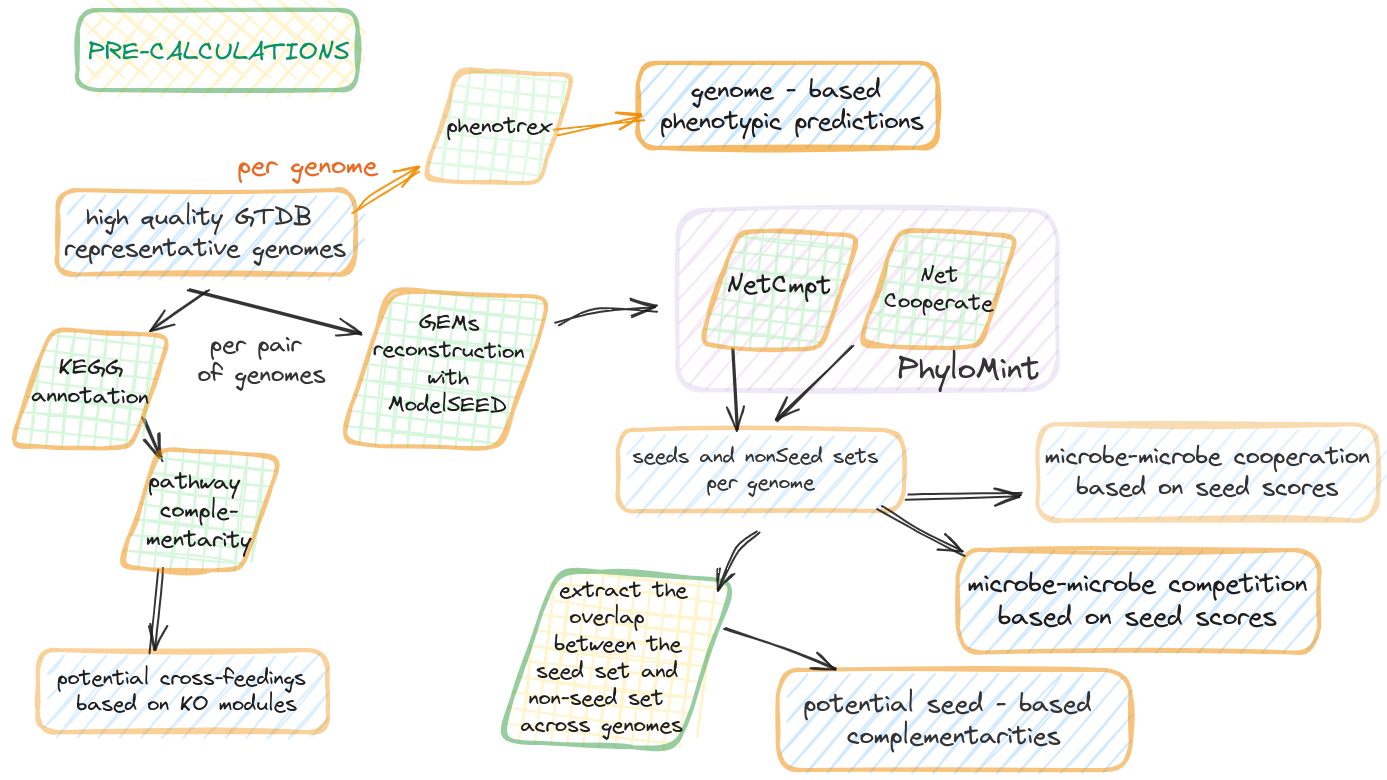
\includegraphics[width=0.9\columnwidth]{figs/microbetag-precal.png}
        \caption{
            Diagram of the \microbetag~pre-calculations.
            % and the on-the-fly workflow (bottom panel). 
            GTDB v207 representative genomes were filtered and for those of high-quality,
            33 phenotypic traits were predicted using~\texttt{phenotrex}.
            To this end, models were re-trained to sync with version 5.0 of eggNOG.
        }
    \end{figure}


    \subsection*{Genomes included}
    \label{subsec:genomes}

        Using the Genome Taxonomy Database (GTDB) v207 \href{https://data.gtdb.ecogenomic.org/releases/release207/207.0/}{metadata files}, we retrieved the NCBI genome accessions of the high-quality representative genomes, i.e., completeness $\geq 95\%$  and contamination $\leq 5\%$.
        % That resulted a set of $26,778$ covering $22,009$ unique NCBI Taxonomy Ids.
        A set of $26,778$ genomes was obtained, representing $22,009$ unique NCBI Taxonomy Ids.
        Using these accession numbers, we were able to download their corresponding \texttt{.faa} files when available 
        % (\href{https://github.com/hariszaf/microbetag/blob/develop/microbetagDB/mappings/gtdb_ncbi/get_gtdb_faa.py}{\texttt{get\_gtdb\_faa.py}}) 
        leading to a set of $16,900$ amino acid sequence files.
        The latter were annotated and used to obtain potential pathway complementarities between pairs of genomes (see paragraph~\ref{subsec:path-compl}).
        Last, when available, their corresponding annotations in the PATRIC database~\cite{wattam2017improvements} were retrieved to reconstruct GENREs~(see paragraph~\ref{subsec:seeds}).


    \subsection*{Taxonomy schemes}
    \label{subsec:taxonomies}

        \microbetag~maps the taxonomy of each entry in the abundance table to their corresponding NCBI Taxonomy Id and, if available, their closest GTDB representative genome(s), since several GTDB representative genomes may map to the same NCBI Taxonomy Id.
        Two well established taxonomy schemes are supported: the GTDB~\cite{parks2022gtdb} that is being broadly used for bins and/or MAGs taxonomic classification and the Silva database~\cite{quast2012silva} that is widely used in amplicon studies. Both taxonomy schemes link their taxonomies to NCBI Taxonomy Ids~\cite{schoch2020ncbi}.
        In case neither of those two taxonomies was used, and the abundance table contains less than 1,000 taxa, \microbetag~maps the user provided taxonomies to the NCBI Taxonomy. 
        %However, this is done only for abundance tables containing less the 1,000 taxa. 
        To this end, \microbetag~makes use of the~\href{https://github.com/seatgeek/thefuzz}{\texttt{fuzzywuzzy}} library that implements the Levenshtein Distance Metric to get the closest NCBI taxon name and thus its corresponding NCBI Taxonomy Id; a high similarity score is used (90) to avoid false positives. 
        Also, using the nodes dump file of NCBI Taxonomy, \microbetag~may retrieve the child taxa of a taxon in user's data, along with their corresponding NCBI Taxonomy Ids, if requested by the user.
        % Thus, \microbetag maps a network taxon to their corresponding NCBI Taxonomy Id and if available their corresponding GTDB genomes.
        If the user provides their abundance table with taxonomies already mapped to the GTDB taxonomy, \microbetag~will report the best possible annotations in a time efficient manner.
        % as it is both time efficient and, mainly, it allows for the best annotations \microbetag could report, it is strongly suggested that both amplicon and shotgun-oriented data to be mapped to GTDB taxonomies.
        
        % Having a taxonomy scheme of GTDB or Silva is mandatory for networks with more than $1,000$ taxa.
        
        % The corresponding taxonomy will be mentioned as "microbetag\_prep".
        
        % There is a great number of taxonomies that are being used in such studies, e.g. Silva~\cite{quast2012silva}, Ribosomal Database Project (RDP)~\cite{cole2014ribosomal}, manually curated ones and more, 
        % As a consequence, there is not a standardised format of the taxonomies assigned, from bioinformatics pipelines used for the analysis of such data.


    \subsection*{Network inference}
    \label{subsec:net-infer}

        When a co-occurrence network is not provided by the user, \microbetag~relies on FlashWeave~\cite{flashweave_cite} to build one on the fly.
        Yet, \microbetag~supports the annotation of networks built from any algorithm/software, in any format Cytoscape can load.

        % a computational approach based on a flexible Probabilistic Graphical Model framework that integrates metadata and predicts direct microbial interactions from heterogeneous microbial abundance data sets with hundreds of thousands of samples. 
        % A flexible Probabilistic Graphical Model framework is used in a computational approach that 
        % incorporates metadata and predicts direct microbial interactions. 
        % This is done using heterogeneous microbial abundance datasets consisting of hundreds of thousands of samples.

        %     •    heterogeneous - enable heterogeneous mode for multi-habitat or -protocol data with at least thousands of samples (FlashWeaveHE)
        %     •    sensitive - enable fine-grained associations (FlashWeave-S, FlashWeaveHE-S), sensitive=false results in the fast modes FlashWeave-F or FlashWeaveHE-F
        %     •    FDR - perform False Discovery Rate correction (Benjamini-Hochberg method) on pairwise associations
        %     •    n_obs_min - don't compute associations between variables having less reliable samples (i.e. non-zero if heterogeneous=true) than this number. -1: automatically choose a threshold.

    \subsection*{\microbetag~pre-processing}
    \label{subsec:preprocess}

        To aid the user to map their sequences to the GTDB taxonomy, DADA2-formatted 16S rRNA gene sequences for both bacteria and archaea~\cite{ali_alishum_2022_6655692} were used to train the IDTAXA classifier of the DECIPHER package~\cite{{murali2018idtaxa}} and are available through the~\href{https:/hub.docker.com/repository/docker/hariszaf/microbetag_prep/}{microbetag preprocess Docker image}.
        Likewise, when the abundance table consists of more than $1,000$ taxa, providing a network as an input is mandatory.
        Again, to help the user, the \microbetag~preprocess Docker image supports the inference of a network using FlashWeave.

        For a computationally efficient way to annotate large networks, a Docker image is provided, so the user runs a taxonomy assignment using the IDTAXA algorithm~\cite{murali2018idtaxa} of the DECIPHER R package~\cite{wright2016using}.
        A co-occurrence network is also built using FlashWeave~\cite{flashweave_cite}, as \microbetag~also does.


    \subsection*{Literature based nodes annotation}
    \label{subsec:fapro}

        Using a set of Tara Ocean samples~\cite{sunagawa2015structure} FAPROTAX~\cite{louca2016decoupling} estimates the functional potential of the bacterial and archaeal communities, by classifying each taxonomic unit into functional group(s) based on the current literature, descriptions of cultured representatives and/or manuals of systematic microbiology. 
        In this manually curated approach, a taxon is associated with a function only if all the cultured species within the taxon have been shown to exhibit that function. 
        % Apparently, FAPROTAX does not support the annotation of clades with no cultured representatives that have been rising thanks to high throughput sequencing technologies.
        % Further, a taxon could be annotated with more than one functions while functional groups could be nested.
        In its current version, FAPROTAX includes more than 80 functions based on ~7600 functional annotations and covers more than 4600 taxa.
        Contrary to gene content based approaches, e.g., PICRUSt2~\cite{douglas2020picrust2}, FAPROTAX  estimates metabolic phenotypes based on experimental evidence. 

        \microbetag~invokes the accompanying script of FAPROTAX and converts the taxonomic microbial community profile of the samples included in the user's abundance table or of the taxa present in the provided network, into putative functional profiles.
        Then, it parses FAPROTAX's sub-tables to annotate each taxonomic unit present in the user's data with all the functions for which they had a hit. 
        FAPROTAX annotations are not part of the microbetagDB but are computed on the fly.


    \subsection*{Genomic based nodes annotation}
    \label{subsec:phen}

        phenDB~\cite{feldbauer2015prediction} is a publicly available resource that supports the analysis of bacterial (meta)genomes to identify 47 distinct functional traits, e.g. whether a species is producing butanol or has a halophilic lifestyle.
        It relies on support vector machines (SVM) trained with manually curated datasets based on gene presence/absence patterns for trait prediction.
        More specifically, the model for a particular trait is trained using a collection of EggNOG annotated genomes where the knowledge of whether that trait is present or absent among its members is available.
        These models (classifiers) are used to predict presence/absence of their corresponding traits in non-studied species. 
        % Based on the completeness/contamination of the genomes, the accuracy varies. 
        % The~\texttt{compute-genotype} program of phenotrex supports the creation of such tabular~\textit{genotype} files.
        % A~\textit{genotype} file can be used along with a~\textit{phenotype} one, i.e., a file containing true phenotypic trait values for each input genome on which to train the model, and the~\texttt{train} program of phenotrex can then be performed. 

        % one can implement tests to evaluate the model based on the completeness of a genomes and its contamination (Performance Estimation) using the cccv program. e.g
        % {
        % 	"mean_balanced_accuracy": 0.5499999999999999,
        % 	"stddev_balanced_accuracy": 0.10482201257840669,
        % 	"contamination": 0.7,
        % 	"completeness": 1.0
        % },
        For microbetagDB, %phenotrex 
        classifiers were re-trained using the genomes provided by phenDB for each trait to sync with the latest version of eggNOG~\cite{huerta2019eggnog} and the~\texttt{phenotrex}~\cite{feldbauer2015prediction} software tool.
        Genomes were downloaded from NCBI using the \href{https://www.ncbi.nlm.nih.gov/sites/batchentrez}{Batch Entrez} program.
        % as there was a conflict between the eggNOG version phenotrex uses at the prediction step and the one during the training of the classes as provided in the PhenDB site.
        % For example, for the acetic acid production case, the corresponding webpage of phenDB pointed to the set of genomes that had been originally used. 
        Then, \textit{genotype} files were produced for all the high quality GTDB representative genomes.
        Each model was then used against all the GTDB \textit{genotype} files to annotate each with the presence or the absence of the trait. 
        A list of all the phenotypic traits available for the genomes present in microbetagDB is available on \microbetag 's \href{https://hariszaf.github.io/microbetag/docs/modules/phen-traits/}{documentation site}.
        The updated models are also available


    \subsection*{Pathway complementarity}
    \label{subsec:path-compl}


        To infer potential pathway complementarities, we consider the modules described in KEGG MODULES database~\cite{keggmodulesdb}.
        % as functional units to highlight can provide a valid proxy.
        A KEGG module is defined as a functional unit within the KEGG framework that represents a set of enzymes and reactions involved in a specific biological process or pathway~\cite{muto2013modular}.
        Such a unit consists of several~\textit{steps}, each of which may have more than one molecular way to occur (Figure~\ref{fig:pathcompl}).
        A module's definition is a logical expression and consists of KOs 
        % and the following symbols:
        that may be coupled with one another as:
            % a. the space, representing a connection in the pathway
            a. connected steps of the pathway
            % b. plus sign, representing a molecular complex,
            b. parts of a molecular complex, 
            % c. comma, representing alternatives and
            c. alternatives of the same step, and 
            % d. minus sign, designates an optional item in the complex.
            d. optional entities of a complex.
        Both (a) and (b) cases should be considered as the~\texttt{AND} logical operator, while (c) would be the~\texttt{OR} (Figure~\ref{fig:pathcompl}).
        Given a module's definition, we will consider as an~\textit{alternative} any subset of the KO terms mentioned in the definition, 
        that has exactly one way to perform each step, provided that all the steps of the module are covered.
        % and support the functioning of all the steps of the module.
        We define a genome as having a~\textit{complete} module, only if all the KOs of at least one alternative are present on it.
        In Appendix~\ref{app:pathcompl} we show an example of a module along with its alternatives.

        Within this framework,~\texttt{kofamscan}~\cite{aramaki2020kofamkoala} was used to annotate with KEGG ORTHOLOGY terms (KOs) the $16,900$ high quality GTDB representative genomes for which a~\texttt{.faa} was available~\cite{kanehisa2012kegg}.
        The KOs of each genome were then mapped to their corresponding KEGG modules; a KO may map to more than one module ($1:n$).
        % , see Appendix~\ref{secA2}).

        \begin{figure}[h!]
            \includegraphics*[width=0.8\columnwidth]{figs/path_complem.png}
            \caption{
                Pathway complementarity approach. 
                The high-quality GTDB genomes were annotated with KEGG ORTHOLOGY (KO) terms.
                The various ways of completing a KEGG module were enumerated and all the possible ways a donor species could "gap-fill" a beneficiary's non-complete module were calculated.
                In this case, there are 4 unique ways to complete the serine biosynthesis module; in all of them K00831 is required.
                However, it is missing from the beneficiary species that supports two out of the three steps of the module's definition.
                A donor species including the missing KO (K00831) could potentially transfer the respective gene or provide the beneficiary species with the relevant intermediary product, enabling the beneficiary species to produce serine.
            }
            \label{fig:pathcompl}
        \end{figure}

        All module definitions were retrieved using the KEGG API and parsed to enumerate their alternatives.
        % (\href{https://github.com/hariszaf/microbetag/blob/develop/microbetagDB/mappings/kegg_mappings/parse_module_definitions.py}{\texttt{parse\_module\_definitions.py}}).
        % A dictionary was built with all the alternatives of each module. 
        %, i.e. alternative sets of KOs, for a module to be complete.
        % (\href{https://github.com/hariszaf/microbetag/blob/develop/microbetagDB/mappings/kegg_mappings/module_definition_map.json}{module\_definition\_map.json})
        Each pair of the KEGG annotated genomes was then investigated for potential pathway complementarities, 
        i.e., whether a genome lacking a number of KOs ($genome_A$) to have a complete module ($module_x$) could benefit from another's species genome(s) ($genome_B$).
        In that case, $genome_B$ does not necessarily have a complete alternative of $module_x$; as long as it has the missing KOs that $genome_A$ needs to complete an alternative of it, $genome_B$ potentially complements $genome_A$ with respect to $module_x$.
        In total, $341,568$ unique complementarities were exported.
        % (\href{https://github.com/hariszaf/microbetag/blob/develop/microbetagDB/scripts/pathway_complementarity.py}{\texttt{pathway\_complementarity.py}})

        Thanks to the graphical user interface (GUI) of the~\href{https://www.kegg.jp/kegg/docs/color_gui.html}{KEGG pathway map viewer}~\cite{kanehisa2020kegg,kanehisa2022kegg}, 
        each complementarity can be visualised as part of the closest KEGG metabolic map; 
        where the KOs contributed by the donor are shown in blue-green whereas those coming from the beneficiary genome are coloured in red.

        \microbetag~annotates the edges of a co-occurrence network by identifying pairs where both taxa map to an annotated genome present in microbetagDB.
        % Each taxon on the network has been mapped to a NCBI Taxonomy Id and their related GTDB genomes.
        Since co-occurrence networks are undirected, both nodes of a suggested association are considered as potential donors and beneficiary species. 
        When more than one GTDB representative genome map to the same NCBI Taxonomy Id all the possible genome combinations are considered.
        Finally, two edges are added in such pairs of taxa in the annotated network: 
        one considering $species_A$ as the potential beneficiary and $species_B$ as the potential donor species, and one vice-versa. 


    \subsection*{Seed scores and complements using genome scale metabolic reconstructions }
    \label{subsec:seeds}

        The Metabolic Complementarity Index ($MI_{Complementarity}$) measures the degree to which two microbial species can mutually assist each other by complementing each other's biosynthetic capabilities.
        As described in~\cite{phylomint_ms}, it is defined as the proportion of seed compounds of a species that can be synthesized by the metabolic network of another but are not included in the seed set of the latter. 
        $MI_{Complementarity}$ offers an upper bound assessment of the potential for cross-feeding interactions between two species.
        Further, the Metabolic Competition Index ($MI_{Competition}$) represents the similarity in two species' nutritional profiles. 
        This index establishes an upper limit on the level of competition that one species may face from another.
        Those indices have been described and implemented in the NetCooperate~\cite{levy2015netcooperate} and NetCompt~\cite{kreimer2012netcmpt} tools respectively.
        We will be referring to those two indices as "seed scores".
        Recently, the~\texttt{PhyloMint} tool~\cite{phylomint_ms} was released supporting the calculation of the seed scores of GENREs in SBML format.

        In the~\microbetag~framework, seed scores were computed using GENREs derived from the high-quality GTDB representative genomes and the~\texttt{PhyloMint} tool.
        GENREs were reconstructed using the Model SEED pipeline~\cite{henry2010high} through its Python interface \href{https://modelseedpy.readthedocs.io/en/latest/index.html}{ModelSEEDpy}.
        The latter requires RAST annotated genomes~\cite{overbeek2014seed}; 
        if available through the PATRIC database~\cite{wattam2017improvements}, annotations were retrieved.
        For the rest of the genomes, RAST annotation was performed through RASTtk~\cite{brettin2015rasttk}.

        Moreover, the computed seed and the non-seed (i.e., metabolic compounds a genome can build on its own) sets of each genome were used to compute their overlap among all the pairwise combinations of those genomes.
        More specifically, seed and non-seed compounds of each genome were mapped to their corresponding KO terms and those related to any KEGG MODULE were considered further.
        Focusing on the KEGG MODULE - related KO terms as terms of interest, the overlap of ${seed\ set}_{species_A}$ with the ${non\ seed\ set}_{species_B}$ was retrieved.
        Such \textit{seed complementarities} were calculated for all pairwise GENREs and are now available through microbetagDB.
        Edges of the co-occurrence network where both taxa have been mapped to at least one GTDB genome can be further annotated mentioning all the KEGG maps for which there is at least one seed compound of the potentially beneficiary species. 



    \subsection*{Clustering network}
    \label{subsec:manta}

        % KF: sentence not complete
        \texttt{manta} is a heuristic network clustering algorithm that clusters nodes within weighted networks effectively, leveraging the presence of negative edges and discerning between weak and strong cluster assignments.
        \microbetag~invokes manta~\cite{rottjers2020manta} to cluster the microbial network.
        In case \texttt{manta} is performed, the annotated network inherits the layout that \texttt{manta} returns.


    \subsection*{The~\microbetag \space  workflow}
    \label{subsec:app}
        % --------------------
        % FIGURE for workflow overall (fig:wf)
        % --------------------
        \begin{figure}[h!]
            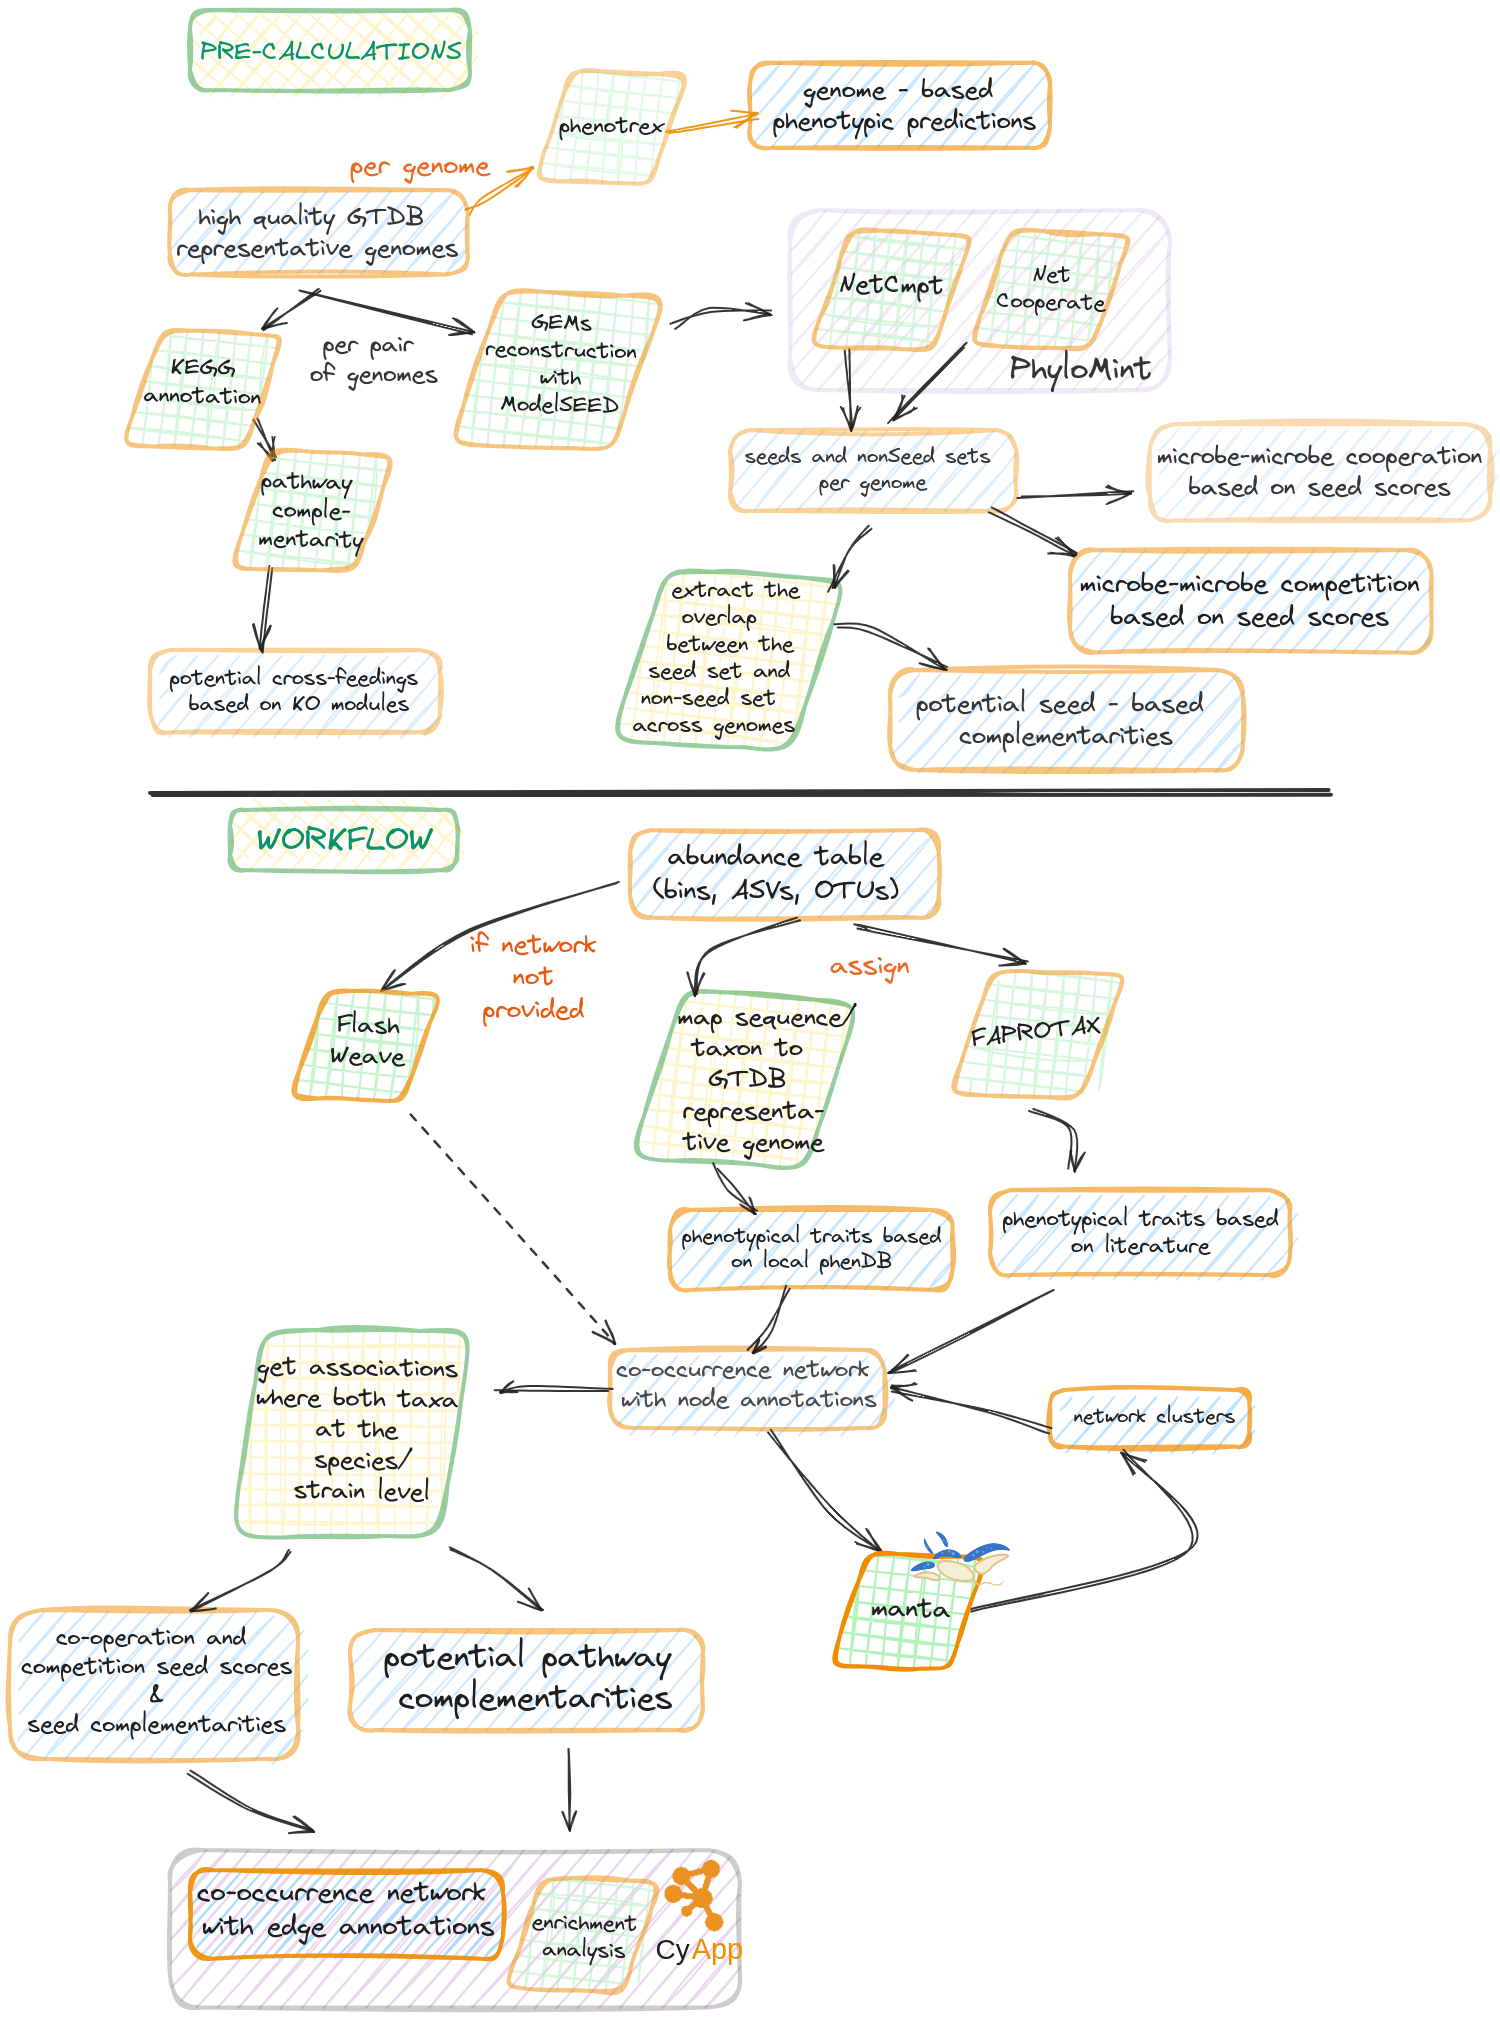
\includegraphics[width=0.9\columnwidth]{figs/microbetag-wf.png}
            \caption{
                Diagram of \microbetag's on-the-fly workflow. 
                \microbetag~expects either an abundance table only as input and infers a co-occurrence network using FlashWeave 
                or an abundance table along with an already inferred co-occurrence network 
                and after mapping taxa present to GTDB reference genomes, for those possible, phenotypic attributes are assigned to the nodes. 
                Literature-based annotations of the nodes are also added using FAPROTAX.
                On the edge level, \microbetag~assigns the pre-calculated potential complements based on the pathway and the seed complementarities approaches. 
                \microbetag~supports optional network clustering with manta.
                The annotated network can then be parsed into Cytoscape using the MGG app.
            }
            \label{fig:wf}
        \end{figure}


        As shown in Figure~\ref{fig:wf}, the~\microbetag~workflow expects an abundance table representing either amplicon or shotgun data.
        If a co-occurrence network is already available, the user may provide it too as input.
        The~\microbetag~workflow will first map the taxa present on the abundance table to their corresponding GTDB representative genomes if that is possible, i.e., in case the taxonomy provided does reach the species or the strain level (see paragraph~\ref{subsec:taxonomies}).
        If a network is not provided, \microbetag~will then build one using FlashWeave~\cite{flashweave_cite}.
        Then the abundance table will be used for a literature-based annotation using FAPROTAX~\cite{louca2016decoupling}.
        This is the only annotation step that is microbetagDB independent within the web-service workflow.
        The nodes of the network will be further annotated with phenotypic traits based on the model predictions~\cite{feldbauer2015prediction}.
        Edges linking taxa assigned to the species or strain level will be annotated with pathway and seed complementarities and seed scores.
        Last, a network clustering will be performed assigning each node to a cluster.
        The annotated network is then returned in a \texttt{.cx} format. 
        The user may skip any of these annotation steps if not needed for their analysis.

        % The~\microbetag workflow is written in Python and can be performed either through the \microbetag API or through the MGG app (see paragraph~\ref{subsec:app}). 
        % It is hosted on the same server as microbetagDB.



    \subsection*{Groups of annotations}
    \label{subsec:groups}

        Biologically meaningful groups were described to group phenotypic traits returned from FAPROTAX and phenDB-like annotation steps.
        The main groups supported are related to: 
        a. the lifestyle of a species, for example being halophilic or thermophyllic etc.,
        b. the biogeochemical processes a species metabolic potential has been found related to, for example Nitrite-oxidizing bacteria (NOB) bacteria and 
        c. important metabolites a species is suggested to produce, e.g. butanol.
        The aim of these groups are to facilitate filtering of the taxa present.
        Enrichment analysis for members of such groups 
        (e.g., based on the clusters identified by an algorithm like \texttt{manta}) 
        can be performed through the CytoscapeApp.


    \subsection*{Software architecture}
    \label{subsec:webserver}


        \microbetag~is a Docker-based application.
        We deployed the \microbetag~application using Docker containers~\cite{merkel2014docker} (v24.0.2)  managed by Docker Compose (see Supplementary Figure~\ref{fig:s1}).
        Docker Compose is a tool for defining and running multi-container Docker applications using a YAML file to configure the services required for the application.
        Containers of three Docker images are being used simultaneously:
        a. a~\href{https://www.mysql.com}{MySQL} database including the microbetagDB
        b. a nginx~\cite{nginx} web server and 
        c. the application itself, including the API and the \microbetag~workflow.
        The latter uses~\href{https://gunicorn.org}{Gunicorn} (20.1.0) to build an application server which communicates with the web server using the Web Server Gateway Interface (WSGI) protocol and handles incoming HTTP requests.
        % Nginx acts as a reverse proxy server that sits in front of Gunicorn and forwards client requests to Gunicorn for processing. It serves as an intermediary between clients and your application server.
        \microbetag~is implemented as a~\href{https://flask.palletsprojects.com/en/3.0.x/}{Flask} application (v2.3.2); 
        Flask is a micro web framework for developing Python web applications and RESTful APIs.
        The API has a route for performing the \microbetag~workflow, either through any Python console or the Cytoscape MGG app, but also several other routes that enable quick and easy access to the microbetagDB content, i.e. the genomes present, their phenotypic traits predicted annotations, pathway and seed complementarities among specific genomes or NCBI Taxonomy Ids and their corresponding seed scores if available.
        % REST stands for Representational State Transfer 
        A thorough description of the \microbetag~API is available at the \href{https://hariszaf.github.io/microbetag/docs/api/}{ReadTheDocs web site}. 
        The source code of the \microbetag~web service is available on~\href{https://github.com/msysbio/microbetagApp/}{GitHub}.


    \subsection*{The \texttt{MGG} CytoscapeApp}
    \label{subsec:build-cytoapp}

        We developed a Cytoscape app to enable a straightforward, user-friendly way to perform the \microbetag~workflow and visualise \microbetag-annotated networks.
        The \microbetag~CytoscapeApp (called \texttt{MGG}) was built based on the~\href{https://github.com/RBVI/scNetViz}{source code} of the scVizNet~\cite{choudhary2021scnetviz}.
        A visual style was developed to facilitate distinguishing annotated nodes and edges.
        Nodes are colored based on the level of the taxonomic assignment with those being annotated highlighted in green.
        Similarly, edges are light green when they carry a positive weight and red when negative. 
        Black edges denote pathway and/or seed complementarities.
        The latter were not accounted for in the edge weights since edges represent an undirected relationship while complementarity/overlap scores assume a direction, i.e. the complementarity score of species A versus B is not necessarily the same as that of B versus A.
        \texttt{MGG} allows the user to import their data, retrieve an annotated network and investigate the annotations through a series of CyPanels both for node and edge annotations.
        Figure~\ref{fig:panels} shows an example of the CyPanels.
        In the node panel (\ref{fig:panels}.A), the node name, the taxonomy as well as the NCBI Taxonomy Id and the GTDB genome to which the sequence was mapped can be viewed. 
        Depending on the user's settings and the available annotations for a node, genomic based predictions may be present and/or literature-based ones.
        Further, the annotation groups mentioned in paragraph~\ref{subsec:groups} are on top of this panel allowing for the selection of the nodes carrying either one among several attributes (OR logical relationship) or all of them (AND).
        Accordingly, in the edges panel (\ref{fig:panels}.B), the beneficiary taxon is specified along with their corresponding GTDB representative sequence identifier.
        Pathway and seed complementarities are shown each in a table.
        Potential metabolic interactions are shown in a sub-table entitled with the genome pair under consideration, as several GTDB genomes may have been assigned to a node.
        In case of pathway complementarities, these tables consist of six columns: a. the KEGG MODULE id of the module to be completed, b. its description, 
        c. a more general metabolic category to which the module belongs,
        d. the complement itself as a list of KEGG terms, 
        e. the alternative that now represents a complete module in the beneficiary and
        f. a URL that points to a coloured KEGG map highlighting the complement.
        If clicked, the user's default browser pops up showing a coloured KEGG map as shown in an example in Figure~\ref{fig:panels}.C.
        Last, MGG allows to test for enrichment or depletion of the phenotypic traits assigned to the nodes in each of the network clusters. 
        Clusters may have been returned from \texttt{manta}~\cite{rottjers2020manta} while performing the \microbetag~workflow or users may assign them on their own or using any other network clustering algorithm.
        For thorough instructions on how to use MGG and \microbetag~the reader may visit the~\href{https://hariszaf.github.io/microbetag/docs/cytoApp/}{ReadTheDocs web site}.

        % The app was based on the StringApp and supported by the NRNB group.
        % -----------
        % MGG CyPanels figure
        % -----------
        \newpage
        \begin{figure}[H]
            \centering
            \includegraphics*[width=0.85\columnwidth]{figs/cyPanel.png}
            \caption{
                CyPanels of the MGG CytoscapeApp. 
                A. \textit{Nodes} panel display the annotations of each taxon (node) mapped to one or more GTDB genomes.
                In this example, genomic predicted phenotypic attributes are shown along with their prediction score.
                B. \textit{Edges} panel displays the list of potential metabolic complementarities between two nodes, specifying which is the potential donor and the potential beneficiary taxon; thus giving a direction to the corresponding edge in the graph. 
                There are two cases of complementarities in \microbetag.
                The first are seed complementarities, which are computed based on the species' reconstructed metabolic networks (case shown above). 
                \textit{Seed complementarities} are first exported based on ModelSEED complements (column three) and mapped in KEGG COMPOUNDS (column four).
                The provided URL points to a colored KEGG map that highlights seeds complementing a beneficiary's metabolic network
                The same applies for the case of the \textit{Pathway complementarities} only there is no ModelSEED ids as they are computed directly from the KEGG annotated genomes and not from the Genome-Scale Metabolic Reconstructions; that is the case for the \textit{Seed complementarities}.
                The second are pathway complementarities. 
                These are directly computed from the KEGG annotated genomes and do not involve ModelSEED ids since the metabolic network construction step is not necessary in this case.
                C. Part of a colored KEGG map returned based on the seed complementarities. 
                Compounds that belong to the beneficiary taxon are colored in cyan while the potential complementing seeds from the donor are highlighted in red.
            }
            \label{fig:panels}
            \thispagestyle{empty} % Remove page number
            \nolinenumbers % Disable line numbering for this page
        \end{figure}


\newpage

% ====================================================
% Results and Discussion 
% ====================================================
\section*{Results and discussion}
\label{sec:results-and-discussion}

    % \footnote{
    %     \textbf{Results-related: }
    %     Significant advance over previously published software (usually demonstrated by direct comparison with available related software)
    %     This should include the findings of the study including, if appropriate, results of statistical analysis which must be included either in the text or as tables and figures. 
    %     This section may be combined with the Discussion section for Software articles.
    %     \textbf{Discussion-related:}
    %     The user interface should be described and a discussion of the intended uses of the software, and the benefits that are envisioned, should be included, together with data on how its performance and functionality compare with, and improve, on functionally similar existing software. 
    %     A case study of the use of the software may be presented. 
    %     The planned future development of new features, if any, should be mentioned.
    %     }

    \subsection*{Annotating microbial co-occurrence networks with \microbetag}
    \label{subsec:running-wf}

        The \microbetag~software ecosystem consists of five main modules:
        a. microbetagDB including~\microbetag~precalculations,
        b. the \microbetag~workflow to annotate the co-occurrence network,
        c. a web server hosting both the~\texttt{microbetagDB} and the~\microbetag~application,
        d. a CytoscapeApp called \texttt{MGG} that enables users to easily invoke the workflow and investigation of the annotated network, and
        e. a stand-alone pre-processing workflow provided as Docker image for data sets with more than $1,000$ sequence identifiers (OTUs/ASVs/bins etc.).

        Currently, microbetagDB includes more than $34,000$ genomes (Table~\ref{tab:db}) along with their corresponding annotations.
        The vast majority of these genomes represent bacterial taxa (364 taxa are Archaea).
        The presence/absence of more than 30 phenotypic traits have been predicted for those genomes.
        About 1.4 billion potential metabolic interactions leading to pathway or seed complementarities have been precomputed as well.
        There are one order of magnitude more seed complements than those corresponding to pathway complementarities as for all GENREs present in microbetagDB all pairwise complements were calculated ($33,755^2$) and stored, even if empty.
        In the case of pathway complementarities, a genome pair is present in the database and thus counted only if a potential complementarity was found.
        Yet, in the first case, the number of genomes with no potential seed complements ranges from zero to a few dozen.
        % A following paper on the microbetagDB content is in preparation.
        All annotations can be accessed directly from microbetagDB through the API.
        Using GENREs for the seed complements rather than the genomes themselves facilitates a more realistic simulation of the essential requirements of corresponding taxa for growth (seeds) and of potential secretions (non-seeds) assuming species (model) growth.
        % and not the genomes per se supports a more realistic simulation of what the corresponding taxa need to get from the environment to grow (seeds) but also, assuming they grow what they may secrete (non-seeds).
        However, this comes with its own challenges (see paragraph~\ref{subsec:pot-and-limits}). 

        Running the \microbetag~workflow is straightforward and can be done using an abundance table with taxonomic assignments as input.
        When the taxonomy scheme being used is not one among the GTDB, Silva or the GTDB-oriented taxonomy for 16S rRNA amplicon data (see pre-process paragraph~\ref{subsec:preprocess}), the most time-consuming step of the workflow is the one mapping user's taxonomy to a NCBI Taxonomy Id and from that to GTDB representative genomes. 
        Network inference can be a computationally intensive step too, particularly as the number of sequences in the abundance table increases. 
        To enable annotation of large data sets, a stand-alone pre-process workflow is provided with \microbetag.
        The user can either assign their amplicon data to the GTDB-oriented taxonomy and/or reconstruct a network locally. 
        Once a network is available and the taxonomy used is among the standard ones for \microbetag, the computational time required for annotation ranges from several seconds to a few minutes based on user's settings.
        An annotated network in \texttt{cx2} format is returned, which can be viewed in Cytoscape.
        A tutorial, frequently asked questions and hints to address the idiosyncrasies of various data sets are available on the~\href{https://hariszaf.github.io/microbetag/}{ReadTheDocs web site} while a Gitter community allows users to exchange experience and ask for more specific help.
        % In the following two sections we present a validation and a use case, highlighting the potential of our approach.
        In the following two sections, we present a validation and use case, highlighting our approach's potential.

        % --------------------
        % TABLE for microbetagDB stats (tab:db)
        % --------------------
        \begin{table}[h!]
            \caption[Summary of Data]{
                Summary of the data in microbetagDB
            }
            \label{tab:db}
            \begin{tabular}{lr}
                \toprule
                Description & Entries \\
                \midrule
                GTDB representative genomes & 34,608 \\
                Phen-model-oriented metabolic functions & 32 \\
                FAPROTAX functions & 92 \\
                Unique pathway complements & 341,568 \\
                Pairwise pathway complementarities & 184,184,548\\
                GENREs & 33,755 \\
                Seed complements & 1,139,400,025\\
                Seed scores & 1,105,250,048 \\
                \bottomrule
            \end{tabular}
        \end{table}


    \subsection*{A validation case}
    \label{subsec:validation}


        To validate \microbetag~we used the correlation network of Hessler et~\textit{al.}~\cite{hessler2023vitamin} describing mine tailing-derived laboratory microbial consortia.
        In this study, \textit{Variovorax}, a thiamine producer, and its co-occurrence with a series of thiamine auxotrophs are discussed.
        The study was selected as a validation case as the authors tested the network's predictions by performing co-culture experiments measuring the thiamine production.
        Sequence bins corresponding to network nodes and the original network were obtained from the authors.
        Using GTDB-tk~\cite{chaumeil2020gtdb}, bins were annotated to GTDB taxonomies; those retrieved were added in the original network, which was then annotated with~\microbetag.
        Supplementary Figure~\ref{fig:s2} highlights bin\_55 that corresponds to \textit{Variovorax} and its first neighbors.
        The annotated network is available on \microbetag's \href{https://github.com/hariszaf/microbetag/blob/develop/tests/validation_case/microbetag_val.cx}{GitHub repository}.
        GTDB-tk returned GCA\_001899795.1 as the one closer to bin\_55 assigning it to \textit{Variovorax} sp001899795.
        \microbetag~then suggested that this specific genome corresponds to an aerobe~\cite{aerobeVariovorax}, that can grow autotrophically if needed~\cite{autotrophVariovorax} and utilizes D-glucose, while producing ethanol and lactic acid~\cite{lacticVariovorax}. 
        Last, the Type VI secretion system was suggested to be available on its genome~\cite{t6ssVariovorax}.

        Hessler et~\textit{al.} argue that \textit{Variovorax} is an important thiamine source and can supply neighboring species that cannot produce it (auxotrophs). 
        Indeed, \microbetag~was able to suggest several thiamine-related potential seed complements among the potential metabolic interactions between \textit{Variovorax} as well as its neighbors (Table~\ref{tab:Variovorax}.A). 
        Potential interactions were also found in some cases between the neighbors themselves (Table~\ref{tab:Variovorax}.B).
        The authors also argue that isolates of that \textit{Variovorax} strain required the addition of pantothenic acid to grow. 
        However, based on the KEGG annotation of the genome that bin\_55 was mapped to, it contains both KEGG MODULES related to pantothenate biosynthesis,  
        M00119 (valine/L-aspartate $\Rightarrow$ pantothenate) and 
        M00913 (2-oxoisovalerate/spermine $\Rightarrow$ pantothenate).
        Other genomes though are not capable of either one or any of those (Supplementary Table)~\ref{tab:VariovoraxGenomes}.
        This example highlights a challenge of the \microbetag~approach (see Section~\ref{subsec:pot-and-limits}). 
        The complementarities between the nodes would have been different if bin\_55 was classified as another \textit{Variovorax} genome, with incomplete modules. 
        For example, if GCF\_001577265.1 was picked and its complementarities with the neighboring taxa were retrieved, it would have revealed that all its neighboring species can actually provide it with pantothenate (C00864) as suggested by their seed complementarities (see
        \href{https://www.kegg.jp/kegg-bin/show_pathway?map00770/C00049%20skyblue%2Cblue/C00099%20skyblue%2Cblue/C00141%20skyblue%2Cblue/C00966%20skyblue%2Cblue/C00010%20skyblue%2Cblue/C00882%20skyblue%2Cblue/C01134%20skyblue%2Cblue/C03492%20skyblue%2Cblue/C04352%20skyblue%2Cblue/C00099%20skyblue%2Cblue/C00141%20skyblue%2Cblue/C00966%20skyblue%2Cblue/C05665%20skyblue%2Cblue/C00010%20skyblue%2Cblue/C00141%20skyblue%2Cblue/C00882%20skyblue%2Cblue/C00966%20skyblue%2Cblue/C01134%20skyblue%2Cblue/C03492%20skyblue%2Cblue/C04352%20skyblue%2Cblue/C18911%20skyblue%2Cblue/C00864%09%23ff0000/C00864%09%23ff0000/C00864%09%23ff0000/}{coloured map}). 


        % C01081: Thiamin monophosphate;
        % \href{https://www.genome.jp/module/M00899+C01081}{Thiamine salvage pathway, HMP/HET => TMP}
        % \href{https://www.genome.jp/module/M00898+C01081}{Thiamine biosynthesis, pyridoxal-5P => TMP/thiamine/TPP}
        % \href{https://www.genome.jp/module/M00897+C01081}{Thiamine biosynthesis, plants, AIR (+ NAD+) => TMP/thiamine/TPP}
        % \href{https://www.genome.jp/module/M00896+C01081}{Thiamine biosynthesis, archaea, AIR (+ NAD+) => TMP/TPP}
        % \href{https://www.genome.jp/module/M00895+C01081}{Thiamine biosynthesis, prokaryotes, AIR (+ DXP/glycine) => TMP/TPP}
        % \href{https://www.genome.jp/module/M00127+C01081}{Thiamine biosynthesis, prokaryotes, AIR (+ DXP/tyrosine) => TMP/TPP}

        % C15809:
        % \href{https://journals.plos.org/plosone/article/figure?id=10.1371/journal.pone.0079786.g005}{thiamine biosynthesis pathway with Iminoglycine }

        % C04327: 4-Methyl-5-(2-phosphooxyethyl)thiazole;
        % C01279: 4-Amino-5-hydroxymethyl-2-methylpyrimidine;
        % \href{https://www.genome.jp/module/M00899+C04327}{thiamine salvage pathway}


        % C20246: 2-[(2R,5Z)-2-Carboxy-4-methylthiazol-5(2H)-ylidene]ethyl phosphate;
        % \href{https://www.genome.jp/module/M00127+C20246}{Thiamine biosynthesis, prokaryotes, AIR (+ DXP/tyrosine) => TMP/TPP}
        % \href{https://www.genome.jp/module/M00895+C20246}{Thiamine biosynthesis, prokaryotes, AIR (+ DXP/glycine) => TMP/TPP}

        % -----------
        % Table for Variovorax - thiamine and neighbors (tab:Variovoraax)
        % -----------
        \begin{table}[ht]
            \begin{minipage}{\linewidth}
                
                \begin{adjustbox}{width=1.3\textwidth,center=\textwidth}
                    \begin{tabular}{c|c}
                        \begin{tabular}{l l l r}
                            \multicolumn{4}{c}{A. \textit{Variovorax} thiamine-related benefits to its neighbors} \\
                            \toprule
                            \thead{Neighboring taxon} & \thead{node id} & \thead{KEGG compounds} & \thead{url} \\
                            \midrule
            
                            \textit{Kapabacteria thiocyanatum}  & bin\_59  &   C15809    &  \href{https://www.kegg.jp/kegg-bin/show_pathway?map00730/C00068%20skyblue%2Cblue/C00082%20skyblue%2Cblue/C01081%20skyblue%2Cblue/C03373%20skyblue%2Cblue/C04556%20skyblue%2Cblue/C04752%20skyblue%2Cblue/C11437%20skyblue%2Cblue/C20246%20skyblue%2Cblue/C00037%20skyblue%2Cblue/C00068%20skyblue%2Cblue/C01081%20skyblue%2Cblue/C03373%20skyblue%2Cblue/C04556%20skyblue%2Cblue/C04752%20skyblue%2Cblue/C11437%20skyblue%2Cblue/C20246%20skyblue%2Cblue/C00003%20skyblue%2Cblue/C00037%20skyblue%2Cblue/C00068%20skyblue%2Cblue/C01081%20skyblue%2Cblue/C03373%20skyblue%2Cblue/C04556%20skyblue%2Cblue/C04752%20skyblue%2Cblue/C00003%20skyblue%2Cblue/C00037%20skyblue%2Cblue/C00068%20skyblue%2Cblue/C01081%20skyblue%2Cblue/C03373%20skyblue%2Cblue/C04556%20skyblue%2Cblue/C04752%20skyblue%2Cblue/C00003%20skyblue%2Cblue/C00018%20skyblue%2Cblue/C00037%20skyblue%2Cblue/C00068%20skyblue%2Cblue/C01081%20skyblue%2Cblue/C04556%20skyblue%2Cblue/C04752%20skyblue%2Cblue/C01081%20skyblue%2Cblue/C04556%20skyblue%2Cblue/C04752%20skyblue%2Cblue/C15809%09%23ff0000/C15809%09%23ff0000/}{url} \\
            
                            \textit{Terrimonas ferruginea}      & bin\_100 &  C15809;C01081    & \href{https://www.kegg.jp/kegg-bin/show_pathway?map00730/C00068%20skyblue%2Cblue/C00082%20skyblue%2Cblue/C03373%20skyblue%2Cblue/C11437%20skyblue%2Cblue/C00037%20skyblue%2Cblue/C00068%20skyblue%2Cblue/C03373%20skyblue%2Cblue/C11437%20skyblue%2Cblue/C00003%20skyblue%2Cblue/C00037%20skyblue%2Cblue/C00068%20skyblue%2Cblue/C03373%20skyblue%2Cblue/C00003%20skyblue%2Cblue/C00037%20skyblue%2Cblue/C00068%20skyblue%2Cblue/C03373%20skyblue%2Cblue/C00003%20skyblue%2Cblue/C00018%20skyblue%2Cblue/C00037%20skyblue%2Cblue/C00068%20skyblue%2Cblue/C01081%09%23ff0000/C15809%09%23ff0000/C01081%09%23ff0000/C15809%09%23ff0000/C01081%09%23ff0000/C01081%09%23ff0000/C01081%09%23ff0000/C01081%09%23ff0000/}{url}  \\
            
                            \textit{Tahibacter} sp001725155     & bin\_167 &  C15809    &  \href{https://www.kegg.jp/kegg-bin/show_pathway?map00730/C00068%20skyblue%2Cblue/C00082%20skyblue%2Cblue/C01081%20skyblue%2Cblue/C03373%20skyblue%2Cblue/C04556%20skyblue%2Cblue/C04752%20skyblue%2Cblue/C11437%20skyblue%2Cblue/C20246%20skyblue%2Cblue/C00037%20skyblue%2Cblue/C00068%20skyblue%2Cblue/C01081%20skyblue%2Cblue/C03373%20skyblue%2Cblue/C04556%20skyblue%2Cblue/C04752%20skyblue%2Cblue/C11437%20skyblue%2Cblue/C20246%20skyblue%2Cblue/C00003%20skyblue%2Cblue/C00037%20skyblue%2Cblue/C00068%20skyblue%2Cblue/C01081%20skyblue%2Cblue/C03373%20skyblue%2Cblue/C04556%20skyblue%2Cblue/C04752%20skyblue%2Cblue/C00003%20skyblue%2Cblue/C00037%20skyblue%2Cblue/C00068%20skyblue%2Cblue/C01081%20skyblue%2Cblue/C03373%20skyblue%2Cblue/C04556%20skyblue%2Cblue/C04752%20skyblue%2Cblue/C00003%20skyblue%2Cblue/C00018%20skyblue%2Cblue/C00037%20skyblue%2Cblue/C00068%20skyblue%2Cblue/C01081%20skyblue%2Cblue/C04556%20skyblue%2Cblue/C04752%20skyblue%2Cblue/C01081%20skyblue%2Cblue/C04556%20skyblue%2Cblue/C04752%20skyblue%2Cblue/C15809%09%23ff0000/C15809%09%23ff0000/}{url}  \\
            
                            \textit{Microbacterium} sp900156455 & bin\_28  &  C15809; C20246  & \href{https://www.kegg.jp/kegg-bin/show_pathway?map00730/C00068%20skyblue%2Cblue/C00082%20skyblue%2Cblue/C01081%20skyblue%2Cblue/C03373%20skyblue%2Cblue/C04556%20skyblue%2Cblue/C04752%20skyblue%2Cblue/C11437%20skyblue%2Cblue/C00037%20skyblue%2Cblue/C00068%20skyblue%2Cblue/C01081%20skyblue%2Cblue/C03373%20skyblue%2Cblue/C04556%20skyblue%2Cblue/C04752%20skyblue%2Cblue/C11437%20skyblue%2Cblue/C00003%20skyblue%2Cblue/C00037%20skyblue%2Cblue/C00068%20skyblue%2Cblue/C01081%20skyblue%2Cblue/C03373%20skyblue%2Cblue/C04556%20skyblue%2Cblue/C04752%20skyblue%2Cblue/C00003%20skyblue%2Cblue/C00037%20skyblue%2Cblue/C00068%20skyblue%2Cblue/C01081%20skyblue%2Cblue/C03373%20skyblue%2Cblue/C04556%20skyblue%2Cblue/C04752%20skyblue%2Cblue/C00003%20skyblue%2Cblue/C00018%20skyblue%2Cblue/C00037%20skyblue%2Cblue/C00068%20skyblue%2Cblue/C01081%20skyblue%2Cblue/C04556%20skyblue%2Cblue/C04752%20skyblue%2Cblue/C01081%20skyblue%2Cblue/C04327%20skyblue%2Cblue/C04556%20skyblue%2Cblue/C04752%20skyblue%2Cblue/C15809%09%23ff0000/C20246%09%23ff0000/C15809%09%23ff0000/C20246%09%23ff0000/}{url}  \\
            
                            \textit{Sphingobium} sp001899715    & bin\_155 &   Iminoglycine C15809;    &  \href{https://www.kegg.jp/kegg-bin/show_pathway?map00730/C00068%20skyblue%2Cblue/C00082%20skyblue%2Cblue/C01081%20skyblue%2Cblue/C03373%20skyblue%2Cblue/C04556%20skyblue%2Cblue/C04752%20skyblue%2Cblue/C11437%20skyblue%2Cblue/C20246%20skyblue%2Cblue/C00037%20skyblue%2Cblue/C00068%20skyblue%2Cblue/C01081%20skyblue%2Cblue/C03373%20skyblue%2Cblue/C04556%20skyblue%2Cblue/C04752%20skyblue%2Cblue/C11437%20skyblue%2Cblue/C20246%20skyblue%2Cblue/C00003%20skyblue%2Cblue/C00037%20skyblue%2Cblue/C00068%20skyblue%2Cblue/C01081%20skyblue%2Cblue/C03373%20skyblue%2Cblue/C04556%20skyblue%2Cblue/C04752%20skyblue%2Cblue/C00003%20skyblue%2Cblue/C00037%20skyblue%2Cblue/C00068%20skyblue%2Cblue/C01081%20skyblue%2Cblue/C03373%20skyblue%2Cblue/C04556%20skyblue%2Cblue/C04752%20skyblue%2Cblue/C00003%20skyblue%2Cblue/C00018%20skyblue%2Cblue/C00037%20skyblue%2Cblue/C00068%20skyblue%2Cblue/C01081%20skyblue%2Cblue/C04556%20skyblue%2Cblue/C04752%20skyblue%2Cblue/C01081%20skyblue%2Cblue/C04556%20skyblue%2Cblue/C04752%20skyblue%2Cblue/C15809%09%23ff0000/C15809%09%23ff0000/}{url} \\
            
                            \textit{Nitrosospira} sp001899235   & bin\_176 &  None  &  None \\
            
                            62-47 sp001899255*                  & bin\_233 &  None  &  None  \\
            
                            \textit{Bosea} sp001898115          & bin\_273 & C04327;C01279 & \href{https://www.kegg.jp/kegg-bin/show_pathway?map00730/C00068%20skyblue%2Cblue/C00082%20skyblue%2Cblue/C01081%20skyblue%2Cblue/C03373%20skyblue%2Cblue/C04556%20skyblue%2Cblue/C04752%20skyblue%2Cblue/C11437%20skyblue%2Cblue/C15809%20skyblue%2Cblue/C20246%20skyblue%2Cblue/C00037%20skyblue%2Cblue/C00068%20skyblue%2Cblue/C01081%20skyblue%2Cblue/C03373%20skyblue%2Cblue/C04556%20skyblue%2Cblue/C04752%20skyblue%2Cblue/C11437%20skyblue%2Cblue/C15809%20skyblue%2Cblue/C20246%20skyblue%2Cblue/C00003%20skyblue%2Cblue/C00037%20skyblue%2Cblue/C00068%20skyblue%2Cblue/C01081%20skyblue%2Cblue/C03373%20skyblue%2Cblue/C04556%20skyblue%2Cblue/C04752%20skyblue%2Cblue/C00003%20skyblue%2Cblue/C00037%20skyblue%2Cblue/C00068%20skyblue%2Cblue/C01081%20skyblue%2Cblue/C03373%20skyblue%2Cblue/C04556%20skyblue%2Cblue/C04752%20skyblue%2Cblue/C00003%20skyblue%2Cblue/C00018%20skyblue%2Cblue/C00037%20skyblue%2Cblue/C00068%20skyblue%2Cblue/C01081%20skyblue%2Cblue/C04556%20skyblue%2Cblue/C04752%20skyblue%2Cblue/C01081%20skyblue%2Cblue/C04556%20skyblue%2Cblue/C04752%20skyblue%2Cblue/C01279%09%23ff0000/C04327%09%23ff0000/}{url}  \\
            
                            54-19 sp001898225**                 & bin\_41  &  C15809   & \href{https://www.kegg.jp/kegg-bin/show_pathway?map00730/C00068%20skyblue%2Cblue/C00082%20skyblue%2Cblue/C03373%20skyblue%2Cblue/C11437%20skyblue%2Cblue/C00037%20skyblue%2Cblue/C00068%20skyblue%2Cblue/C03373%20skyblue%2Cblue/C11437%20skyblue%2Cblue/C00003%20skyblue%2Cblue/C00037%20skyblue%2Cblue/C00068%20skyblue%2Cblue/C03373%20skyblue%2Cblue/C00003%20skyblue%2Cblue/C00037%20skyblue%2Cblue/C00068%20skyblue%2Cblue/C03373%20skyblue%2Cblue/C00003%20skyblue%2Cblue/C00018%20skyblue%2Cblue/C00037%20skyblue%2Cblue/C00068%20skyblue%2Cblue/C15809%09%23ff0000/C15809%09%23ff0000/}{url}   \\
            
                            \textit{Rhodoglobus} sp001725325    & bin\_8   &  C15809  & \href{https://www.kegg.jp/kegg-bin/show_pathway?map00730/C00068%20skyblue%2Cblue/C00082%20skyblue%2Cblue/C01081%20skyblue%2Cblue/C03373%20skyblue%2Cblue/C11437%20skyblue%2Cblue/C00037%20skyblue%2Cblue/C00068%20skyblue%2Cblue/C01081%20skyblue%2Cblue/C03373%20skyblue%2Cblue/C11437%20skyblue%2Cblue/C00003%20skyblue%2Cblue/C00037%20skyblue%2Cblue/C00068%20skyblue%2Cblue/C01081%20skyblue%2Cblue/C03373%20skyblue%2Cblue/C00003%20skyblue%2Cblue/C00037%20skyblue%2Cblue/C00068%20skyblue%2Cblue/C01081%20skyblue%2Cblue/C03373%20skyblue%2Cblue/C00003%20skyblue%2Cblue/C00018%20skyblue%2Cblue/C00037%20skyblue%2Cblue/C00068%20skyblue%2Cblue/C01081%20skyblue%2Cblue/C01081%20skyblue%2Cblue/C15809%09%23ff0000/C15809%09%23ff0000/}{url} \\
                            \bottomrule
                        \end{tabular} &
                        \begin{tabular}{ccc}
                            \multicolumn{3}{c}{B. Potential thiamine-related complements among \textit{Variovorax} neighbors} \\
                            \toprule
                            \thead{Beneficiary} & \thead{Donor} & \thead{potential complement} \\
                            \toprule
                            \textit{T. ferruginea} & \textit{Tahibacter} sp001725155 & C01081 \\
                            \textit{T. ferruginea} & \textit{Rhodoglobus} sp001725325 & C01081 \\
                            \textit{Nitrosospira} sp001899235 & \textit{Bosea} sp001898115 & C04327;C01279 \\
                            Chloroflexi & \textit{Bosea} sp001898115 & C15809 \\
                            Chloroflexi & Xanthobacteraceae & C15809 \\
                            Chloroflexi & \textit{Nitrosospira} sp001899235 & C15809 \\
                        \end{tabular} \\
                    \end{tabular} \\
                \end{adjustbox}
            \caption{ 
                Thiamine biosynthesis related seed complements between \textit{Variovorax} and its first neighbors in the network of Hessler \textit{et al.}\cite{hessler2023vitamin} (A), and between pairs of the neighbors (B).
                Bin sequence files were mapped against GTDB using GTDB-tk. 
                Chloroflexi refers to the GTDB taxonomy of: 54-19 sp001898225
            }
            \label{tab:Variovorax}
            \end{minipage}
            \end{table}
    
        % --- end of large table with urls ---
    




        % From the hub species: 
        % \begin{itemize}
        %         node        taxonomy                                role 
        %     \item bin\_54  d\_\_Bacteria;p\_\_Proteobacteria;c\_\_Alphaproteobacteria;o\_\_Acetobacterales;f\_\_Acetobacteraceae;g\_\_70-18;s\_\_70-18 sp001899585
        %     \item bin\__55 s__Variovorax sp001899795 serves thiamine 
        %     \item bin\_116 Novosphingobium sp001898925
        %     \item bin\_176 Nitrosospira sp001899235   
        %     \item bin\_206 Mesorhizobium sp001899205
        %     \item bin\_215 d\_\_Bacteria;p\_\_Proteobacteria;c\_\_Gammaproteobacteria;o\_\_Xanthomonadales;f\_\_Rhodanobacteraceae;g\_\_66-474;s\_\_66-474 sp001899805
        %     \item bin\_221 Chitinophagaceae;g\_\_Palsa-955;s\_\_     not a genome 
        %     \item bin\_261 Comamonas C sp001725255         GTDB genome that would be assigned \href{https://gtdb.ecogenomic.org/genome?gid=GCA_001725255.1}{GCA_001725255.1} but has a completeness of 94.59\%

        % \end{itemize}



    \subsection*{Interpreting a real-world network with \microbetag}
        \label{subsec:usecase}


        Annelies' dataset. 

        One last visual component from the use case would be nice to have.  





    \subsection*{Potential and limitations}
    \label{subsec:pot-and-limits}

        The previous paragraph shows the potential of \microbetag~in the interpretation of co-occurrence networks and how it can be used to generate new hypotheses derived from those.
        However,~\microbetag~benefits the microbiome community in several other ways. 
        The microbetagDB provides a vast number of annotations; 31 predicted traits for more than $30,000$ genomes, their GENREs along with their corresponding seed sets, potential metabolic complementarities and cooperation/competition scores.
        Such a resource may support a range of studies; 
        from a more theoretical perspective regarding the distribution of the complements among taxonomic groups or how often a complement potentially appears, to applications such as eco-evolutionary studies and the investigation of interactions.

        Yet, there are several challenges involved in our approach.
        First, \microbetag~inherits all the biases and drawbacks of both the data and the software it is based on.
        Functional annotation comes with its own limitations.
        Some domains boast richer annotations and more comprehensive descriptions compared to others, thus exhibiting a wealth of detail and employing more precise terminology, particularly for widely recognized processes~(e.g., glycolysis and secondary metabolites biosynthesis correspondingly).

        In the validation case, the bin representing the \textit{Variovorax} strain was mapped to a genome that is supposed to contain the pantothenate KEGG modules.
        Thus, the fact that it requires to receive pantothenate from its environment to grow, as the authors mention, would not have been predicted in the \microbetag~framework. 
        Beyond the sequencing and the annotation challenges, we also need to consider the fact that a pathway may not be fully represented in a KEGG module.
        Of course, various factors can prevent the actual production of an enzyme even if its genetic information is included in a species' genome.
        % , including genetic mutations, regulatory mechanisms, or environmental conditions 
        
        Pathway complementarity can only be as accurate as the KEGG MODULE database and as precise as  the software annotating genomes with KO terms.
        It is well known that automated Genome-Scale Metabolic Reconstruction comes with a great number of challenges and different software for this task come with their intrinsic limitations~\cite{mendoza2019systematic}. 
        Using ModelSEED with a complete medium may limit potential metabolic interactions but, on the other hand, the retrieved ones will be of higher confidence.
        % reconstructing GENREs with automatic tools is of course a challenging tasks and it is known that comes with several drawbacks that especially when producing reconstructions massively

        It is also well known that higher-order interactions, i.e. interactions involving more than two species~\cite{zelezniak2015metabolic}, should also be considered.
        % can reshape microbial interactions~\cite{morin2022higher}. 
        Pairwise relationships do not capture the more complex forms of ecological interactions, in which species depend on (or are influenced by) multiple other species~\cite{faust2012microbialReviewInteractions}.
        However, since \microbetag~is decoupled from network inference, it could annotate a network with hyperedges (i.e. edges connecting more than two taxa) produced by a future tool capable of inferring higher-order interactions.

        Last, the limited number of Archaea in microbetagDB is also the result of a software limitation.
        As shown in~\cite{chklovski2023checkm2} (Figure 6b), the original version of CheckM~\cite{parks2015checkm} that is still being used by GTDB returns lower completeness scores for genomes that correspond to phyla known for having smaller genomes in general, 
        e.g. Patescibacteria representative genomes on GTDB have an average completeness of $\sim 65\%$.
        Thus, only few representatives from these taxonomic groups passed our filters leading to an important under-representation of Archaea.


    \subsection*{Future work}
    \label{subsec:future}

        In the near future, we plan to develop two main features: 
        a. the integration of transcriptomics data provided by the user, which would enhance or lower the probability for a potential metabolic interaction to occur based on whether the KO terms involved are present or not, and 
        b. the integration of spatial data; it is well-known that 
        % the spatial dimension 
        the distance between cells 
        % plays a great role to the extent that an 
        determines whether an 
        interaction occurs~\cite{dal2020short}.
        For this, we intend to support data with 
        % user's data on how their data are distributed in space
        spatial dimensions. 
        Thus, potential metabolic interactions between taxa that are closer to one another would be more probable to occur.

        % Last, we already work on a \textit{"for advanced users"} version, a server-independent version of \microbetag is about to be released, so the user can provide bins/MAGs of theirs and annotations will be made not by mapping taxonomies to reference genomes but using their sequencing data directly.
        % This would require important computing resources and time and cannot be supported in an app-framework like the one presented here. 
        % In this case, one will be again able to investigate the annotated network returned through Cytoscape and the MGG app.
        % \footnote{Could be part of this release; time will tell.}

        % Further indices using the seed concept have been also presented such as the metabolic interaction potential ($MIP$) and the metabolic resource overlap ($MRO$).
        % $MIP$ is defined as the difference between the minimal number of components required for the growth of all members in a noninteracting community and an interacting community, i.e. the maximum number of essential nutritional components that a community can provide for itself through interspecies metabolic exchanges~\cite{zelezniak2015metabolic}.
        % Similarly, $MRO$ is defined as the maximum possible overlap between the minimal nutritional requirements of all member species~\cite{zelezniak2015metabolic}.
        % Regression and association rule mining~\cite{assocciationRuleMining} can be applied to address this challenge.



% ====================================================
% Conclusions
% ====================================================
\section*{Conclusions}
\label{sec:conclusions}

    % \footnote{
    %   This should state clearly the main conclusions and provide an explanation of the importance and relevance of the case, data, opinion, database or software reported.
    % }

    Co-occurrence networks are widely used in microbiome studies to explore associations~\cite{rottjers2018hairballs}. 
    However, their inference and their interpretation come with a range of challenges~\cite{faust2021open}.
    Metabolic exchanges among microbial taxa are considered ubiquitous~\cite{kost2023metabolic} n a large number of environments. 
    In our study, we exploit reverse-ecology approaches and publicly available genomic data and software to predict phenotypic traits and construct metabolic networks to annotate co-occurrence networks derived from amplicon or shotgun data.
    Our annotation was in-line with the study of Hessler et \textit{al.}~\cite{hessler2023vitamin} predicting thiamine-related metabolic interactions among \textit{Variovorax} and its closest neighbors, suggesting several ways to achieve them. 
    Using ..... \todo{Use case}
    Enrichment analysis using them combined with network clustering algorithms can further benefit their interpretation.
    Both microbetagDB and \microbetag~will benefit microbiome studies, as a resource and as a hypothesis generation tool.

\backmatter



\bmhead{Supplementary information}
\label{supplementary-files}
    
    List of supplementary figures and tables.

    \textbf{Supplementary Figure 1:} \microbetag~software ecosystem architecture.

    \textbf{Supplementary Figure 2:} \textit{Variovorax} (node\_55) and its closest neighbors. \textit{Variovorax} annotations are shown in the node CyPanel.

    \textbf{Supplementary Table 1:} \textit{Variovorax} genomes present on microbetagDB and their corresponding complete/incomplete presence of the pantothenate - 
    related KEGG modules

    \textbf{Supplementary Table 2:} Computing times per step of the \microbetag~workflow using four different data sets. 



% ====================================================
% Declarations
% ====================================================
\section*{Declarations}


    \begin{itemize}

        \item \textbf{Availability of data and materials}

            \begin{itemize}
                \item Raw sequences for the use case: 
                \item Raw data for the validations case:
            \end{itemize}

        \item \textbf{Funding}
        
            This work was initiated thanks to an EMBO Scientific Exchange Grant to HZ. 
            It was then supported by the 3D’omics Horizon project (101000309). 
            We would also like to thank the National Resource for Network Biology (NRNB) and the Google Summer of Code 2023 for the support of E.I.M.D.

        \item \textbf{Conflict of interest/Competing interests} 

            The authors declare that they have no other competing interests.

        \item \textbf{Authors' contributions}

            Conceptualization: K.F.
            Methodology: K.F. and H.Z.
            Software: H.Z., E.I.M.D. and J.M.
            Validation: H.Z. and K.F.
            Formal analysis: H.Z. and K.F.
            Investigation: H.Z.
            Resources: K.F., A.E. and A.G.
            Data Curation: H.Z.
            Writing - Original Draft: H.Z. and K.F. 
            Writing - Review \& Editing: all
            Visualization: H.Z.
            Supervision: K.F., H.Z. and S.M.
            Project administration: K.F.
            Funding acquisition: K.F., H.Z.


        \item \textbf{Acknowledgements}

            We would like to thank Dr. Christina Pavloudi for the insight on how to organise the trait groups.
            We would also like to thank Dr. Hessler and Prof. Jillian F. Banfield for sharing both the bins and the network of their study~\cite{hessler2023vitamin}. 


        \item \textbf{Ethics approval}

            Not applicable

        \item \textbf{Consent to participate}
        
            Not applicable.

        \item \textbf{Code availability: }

            \begin{itemize}
                \item microbetagDB related scripts: \href{https://github.com/hariszaf/microbetag}{https://github.com/hariszaf/microbetag}
                \item \microbetag~application: \href{https://github.com/msysbio/microbetagApp}{https://github.com/msysbio/microbetagApp}.
                \item MGG CytoscapeApp: \href{https://github.com/ermismd/MGG/}{https://github.com/ermismd/MGG/}
                \item Validation and use case: 
                % \footnote{Consider moving that under the 3D'omics organization}
                \item Documentation web-site: \href{https://hariszaf.github.io/microbetag/}{https://hariszaf.github.io/microbetag/}
            \end{itemize}

    \end{itemize}


% ====================================================
% Appendices
% ====================================================
\begin{appendices}

    % \subsection*{Background on seed scores}
    % \label{app:seeds}


        % In that case, once a seed is assured, it activates all the rest of that group.
        % Therefore, a confidence level ($C$) ranging from 0 to 1, has been previously described to quantify the relevance of each seed:

        % \begin{equation}
        %     \label{eq:confidence}
        %     C_i = 1 / seed's\ group\ with \ i \ size
        % \end{equation}

        % $C=0$ corresponds to a non-seed node, while $C=1$ represents an independent node. 



        % \begin{equation}
        %     \label{eq:mi_complementarity}
        %     MI_{Complementarity} = \frac{ | SeedSet_A \cap \neg SeedSet_B | }{ | SeedSet_A \cap (SeedSet_B \cup \neg SeedSet_B) | }
        % \end{equation}


        % As also described in~\cite{phylomint_ms}, it is calculated as the proportion of compounds in a species' seed set that coincide with those in an other's, while also factoring in the confidence scores associated with seed compounds.

        % \begin{equation}
        %     \label{eq:mi_competition}
        %     MI_{Competition} = \frac{ \sum C (SeedSet_A \cap SeedSet_B) }{ \sum{ C (SeedSet_A )} }
        % \end{equation}


    \section{Background on pathway and seed complementarity}
    \label{app:pathcompl}

        For a genome to have a KEGG module~\textit{complete} means it provides at least one complete~\textit{alternative}.
        % Based on the module's definition, alternatives are considered as the unique combinations of KOs that will enable the module.
        Alternatives are considered as the unique combinations of KOs that connect an input compound to an output compound of the module 
        For example, the definition of the D-Galacturonate degradation in Bacteria (\href{https://www.genome.jp/dbget-bin/www_bget?M00631}{M00631}) is:
        \bigskip
        \begin{verbatim}    K01812 K00041 (K01685,K16849+K16850) K00874 (K01625,K17463)\end{verbatim}
        \bigskip
        
        Once breaking down, it leads to 4 alternative sets of KOs (pathways):

        \bigskip
        \begin{verbatim}
        K01812 K00041 K01685 K00874 K01625
        K01812 K00041 K16849+K16850 K00874 K01625
        K01812 K00041 K01685 K00874 K17463
        K01812 K00041 K16849+K16850 K00874 K17463
        \end{verbatim}
        \bigskip

        In alternatives two and four, the K16849+K16850 is a \textit{complex}, meaning both KO terms are required for the step to be available.

        In case of seed complementarity, in \microbetag~we focus on the effect that a metabolic exchange between two taxa might have if the seed of the beneficiary taxon is linked to a KEGG MODULE.
        Therefore, the KOs that were found linked to modules were mapped to ModelSEED ids. 
        The initial seed and non-seed sets that were exported as sets of ModelSEED ids were then mapped to KOs too.
        % When the non-seed set of a genome (donor) was able to provide a seed that is related to a KEGG module to another genome (beneficiary) was considered as potential metabolic interaction.
        When the non-seed set of a genome (donor) provided a seed related to a KEGG module to another genome (beneficiary), this is considered a potential metabolic interaction.


    \clearpage
    \section{Validation}
    \label{app:val}

        % Variovorax genomes Table - (tab:VariovoraxGenomes)
        \begin{table}[h!]
            \caption{
                \textit{Variovorax} genomes present in microbetagDB and their corresponding complete/incomplete presence of the pantothenate-related KEGG modules.
                The genome that bin\_55 was mapped to is shown in bold.
            }
            \label{tab:VariovoraxGenomes}
            \begin{tabular}{rrr}
                \thead{Genome}  & \thead{md:M00119} & \thead{md:M00913} \\
                \toprule
                GCA\_004210915.1 & incomplete             & complete                   \\
                GCA\_902506565.1 & incomplete             & incomplete                 \\
                GCF\_000184745.1 & complete               & complete                   \\
                GCF\_000282635.1 & complete               & complete                   \\
                GCF\_000463015.1 & complete               & complete                   \\
                GCF\_000834655.1 & complete               & complete                   \\
                GCF\_001424835.1 & complete               & complete                   \\
                GCF\_001425205.1 & complete               & complete                   \\
                GCF\_001426505.1 & complete               & complete                   \\
                GCF\_001577265.1 & incomplete             & incomplete                 \\
                GCF\_002157355.1 & complete               & complete                   \\
                GCF\_002754375.1 & complete               & complete                   \\
                GCF\_003019815.1 & incomplete             & complete                   \\
                \textbf{GCA\_001899795.1} & \textbf{complete}    &   \textbf{complete} \\
                GCF\_003852515.1 & complete               & complete                   \\
                GCF\_003951285.1 & complete               & complete                   \\
                GCF\_003952165.1 & complete               & complete                   \\
                GCF\_003952185.1 & complete               & complete                   \\
                GCF\_003984625.1 & complete               & complete                   \\
                GCF\_003984645.1 & complete               & complete                   \\
                GCF\_006438845.1 & complete               & complete                   \\
                GCF\_007828835.1 & complete               & complete                   \\
                GCF\_009498455.1 & complete               & complete                   \\
                GCF\_009755665.1 & complete               & complete                   \\
                GCF\_010499245.1 & complete               & complete                   \\
                GCF\_013376045.1 & complete               & complete                   \\
                GCF\_014170375.1 & complete               & complete                   \\
                GCF\_014302995.1 & complete               & complete                   \\
                GCF\_014303735.1 & incomplete             & incomplete                 \\
                GCF\_901827175.1 & complete               & complete                   \\ 
                GCF\_901827205.1 & complete               & complete              
            \end{tabular}
        \end{table}

        % Figure for architectire - (figs:s1)
        \begin{figure}[H]
            \includegraphics*[width=0.9\columnwidth]{figs/architecture.png}
            \caption{
                % \microbetag~software ecosystem. 
                \microbetag~software ecosystem. 
                Three Docker containers are combined: 
                a nginx web server connected to a MySQL database and the \microbetag~workflow.
                An API, as part of the last container, enables the communication between the client (front) and the server side (back end).
                The content of the microbetagDB and the \microbetag~workflow are accessible through a web-browser, a terminal and a CytoscapeApp (MGG).
            }
        \label{fig:s1}
        \end{figure}
    
        % Figure for Variovorax - (fig:s2)
        \begin{figure}[H]
            \includegraphics*[width=0.9\columnwidth]{figs/node55Neigh.png}
            \caption{
                \textit{Variovorax} node (bin\_55) and its neighbors annotated by \microbetag. 
                All but three of them were not mapped to a GTDB representative genome. 
                Green edges represent the positive association weights. 
                The black edges represent pairwise seed complementarities and scores.
            }
            \label{fig:s2}
        \end{figure}
        

        % Time performance using various datasets 
        % % -----------
        % % stats table
        % % -----------
        % \begin{table}[h!]
        %     % \centeringe
        %     \begin{adjustbox}{width=1.3\textwidth,center=\textwidth}

        %         \begin{tabular}{c|c}
        %             \begin{tabular}{ccc}
        %                 \multicolumn{3}{c}{A. GTDB-tk: 480 bins} \\
        %                 \toprule
        %                 \thead{Step} & \thead{Time (sec)} & \thead{Notes} \\
        %                 \toprule
        %                 % \makecell[tl]
        %                 {Taxonomy } & Cell 1,2 & on the fly\\
        %                 {Network } & Cell 2,2 & on the fly\\
        %                 {microbetag} & Cell 3,2 & on the fly\\
        %                 {manta clustering} & Cell 4,2 & \\
        %             \end{tabular} &
        %             \begin{tabular}{ccc}
        %                 \multicolumn{3}{c}{B. GTDB 16S: 3000 ASVs} \\
        %                 \toprule
        %                 \thead{Step} & \thead{Time (sec)} & \thead{Notes} \\
        %                 \toprule
        %                 {Taxonomy assignment*} & & \\
        %                 {Taxonomy mapping}  & & \\
        %                 {Network inference} & & \\
        %                 {microbetag annotations} & & \\
        %                 {manta clustering} & & \\
        %             \end{tabular} \\
        %             \\
        %             \hline
        %             \\
        %             \begin{tabular}{ccc}
        %                 \multicolumn{3}{c}{C. Silva: } \\
        %                 \toprule
        %                 \thead{Step} & \thead{Time (sec)} & \thead{Notes} \\
        %                 \toprule
        %                 {Taxonomy mapping} & & \\
        %                 {Network inference} & & \\
        %                 {microbetag annotations} & & \\
        %                 {manta clustering} & & \\
        %             \end{tabular} &
        %             \begin{tabular}{ccc}
        %                 \multicolumn{3}{c}{D. fuzzywuzzy: } \\
        %                 \toprule
        %                 \thead{Step} & \thead{Time (sec)} & \thead{Notes} \\
        %                 \toprule
        %                 {Taxonomy mapping } & & \\
        %                 {Network inference} & & \\
        %                 {microbetag annotations } & & \\
        %                 {manta clustering } & & \\
        %             \end{tabular} \\
        %         \end{tabular}
        %     \end{adjustbox}
        %     \captionsetup{justification=centering} %
        %     \caption{
        %         Computing times per step using an abundance table of 400 taxa with taxonomy: 
        %         A. taxonomy scheme 
        %         B. 
        %         C.
        %         D. 
        %         *specs of the laptop used.
        %         Docker image on HP*
        %     }
        %     \label{sup.tab:times}
        % \end{table}


        \clearpage





\end{appendices}


% ======================
% Bibliography
% ======================
\newpage
\bibliography{sn-bibliography}


\end{document}

